\chapter{APP AS A DATA ANALYSIS TOOL}
\label{chap:analysis_tool}

\textbf{Data analysis} is a procedure used to examine, clean, change and rebuild information with a view to reach to a specific decision for a given circumstance. Information investigation is normally of two sorts: subjective or quantitative. The sort of information directs the technique for examination. In subjective research, any non-numerical information like content or individual words are broke down. Quantitative examination, then again, centers around estimation of the information and can utilize insights to help uncover results and ends. The outcomes are numerical. At times, the two types of examination are utilized as an inseparable unit. For instance, quantitative investigation can help demonstrate subjective ends. Spatial information investigation is concerned about that part of information examination where the land referencing of articles contains imperative data. This chapter talks about the ways this app can be used as an analysis tool directly or indirectly. \\

\section{Data downloading}

\textbf{Downloading} is defined as the transfer of data from server to your system or belonging. In other words, it is defined as the transmission of data from one machine to another. The significant advantage of downloading is that it gives you the full power over the information with the goal that you can utilize that information. The app gives you the feature of exporting any admim level (0, 1 or 2) data in \gls{csv} format via email option so that it can be used in any form of spatial analysis. Process of data downloading is described below.

\begin{itemize}
    \item Select year, date and tap on country to see the data and then tap on any region. Once you do that, you will see two buttons on both top corners of the screen. Figure 5.1 shows the two buttons which appears after having valid data on globe / map. \\
    
      \begin{figure}[H]
            \centering
            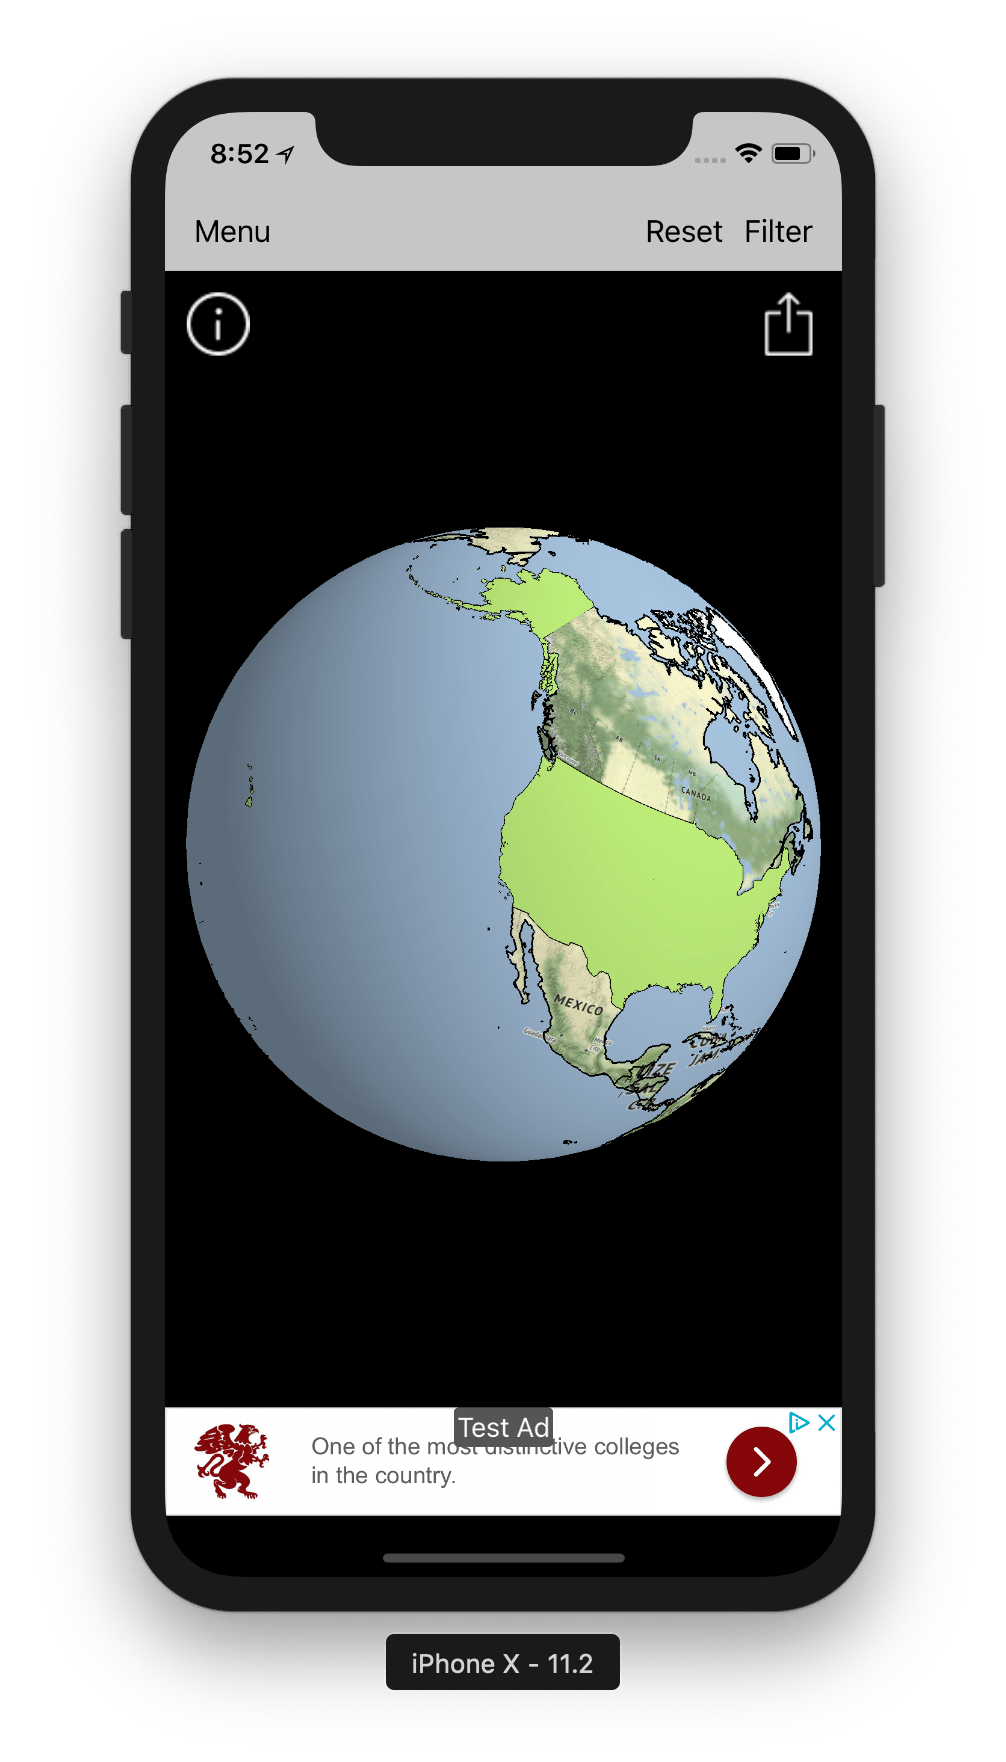
\includegraphics[width=0.25\linewidth]{figures/ch5/buttons.png}
            \caption{\label{fig:buttons} Home screen with two buttons on top corners}
        \end{figure}
     
    \item Left button in figure 5.1 corresponds to Info button which shows information about the current data that is being displayed. Figure 5.2 shows the view appears on tapping of information button. \\
    
      \begin{figure}[H]
            \centering
            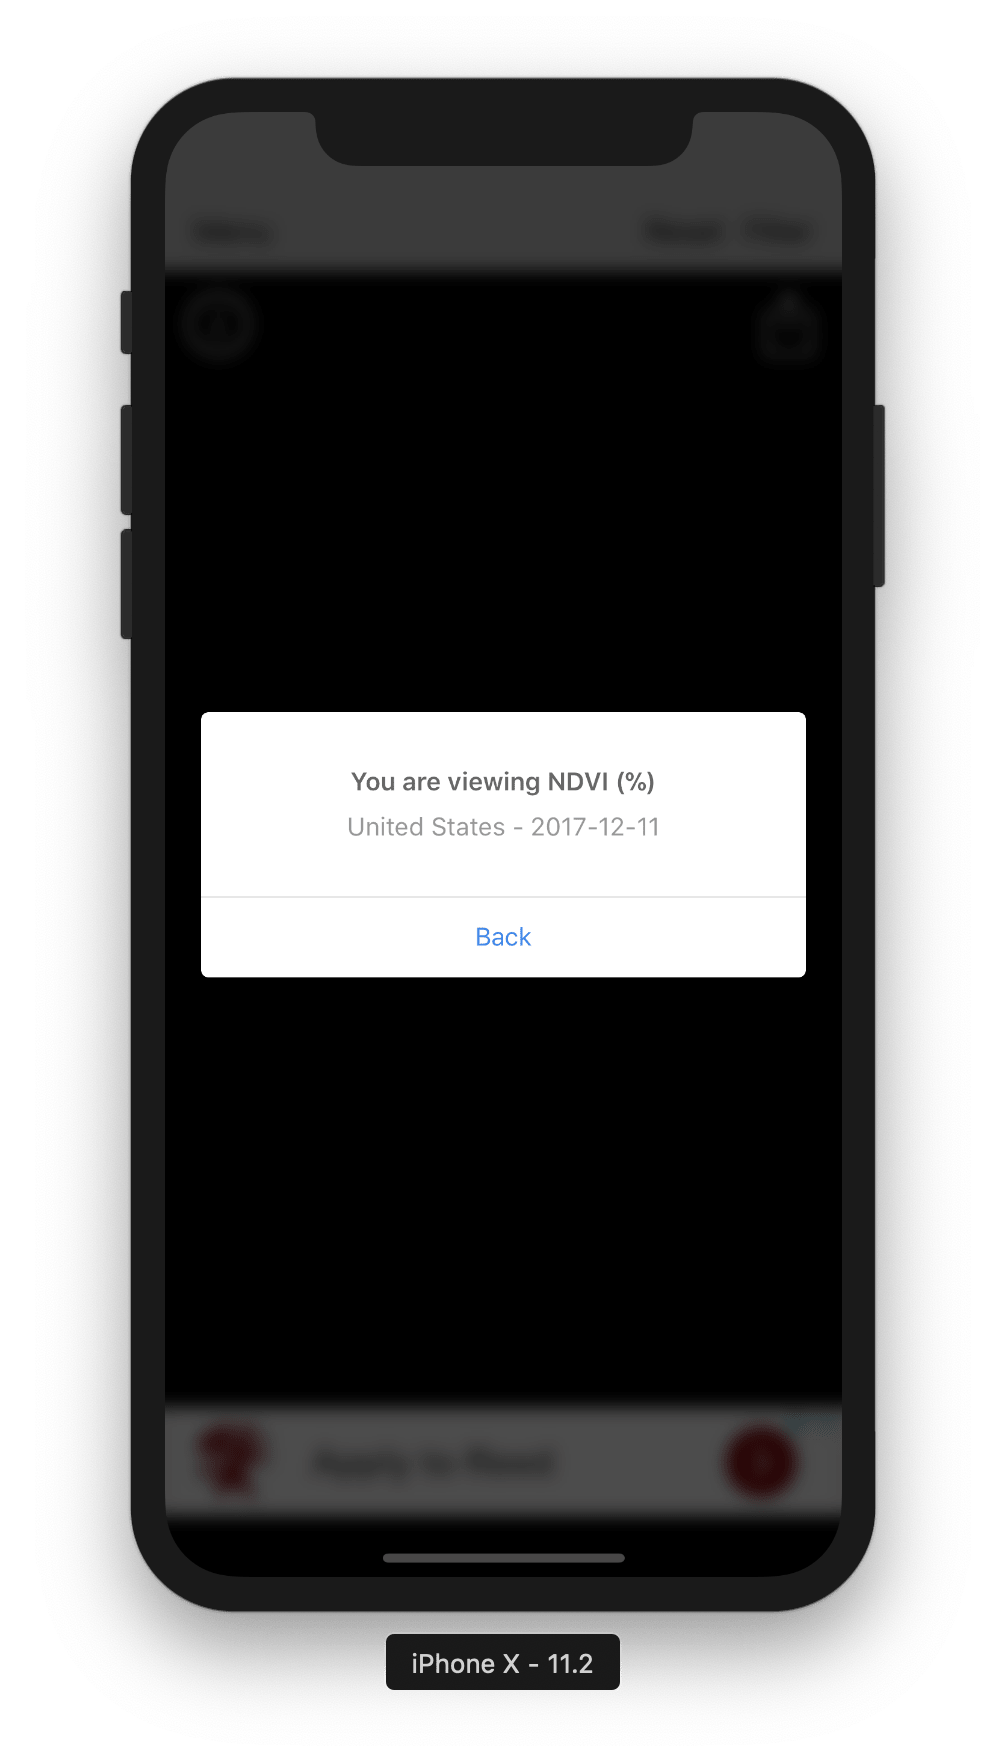
\includegraphics[width=0.25\linewidth]{figures/ch5/info_view.png}
            \caption{\label{fig:info_button} Information button action}
        \end{figure}
       
     \item Right button in figure 5.1 corresponds to export button which prompts you for exporting current data which is visible on globe / map. Figure 5.3 shows the export view on tapping of export button. \\
     
     \begin{figure}[H]
            \centering
            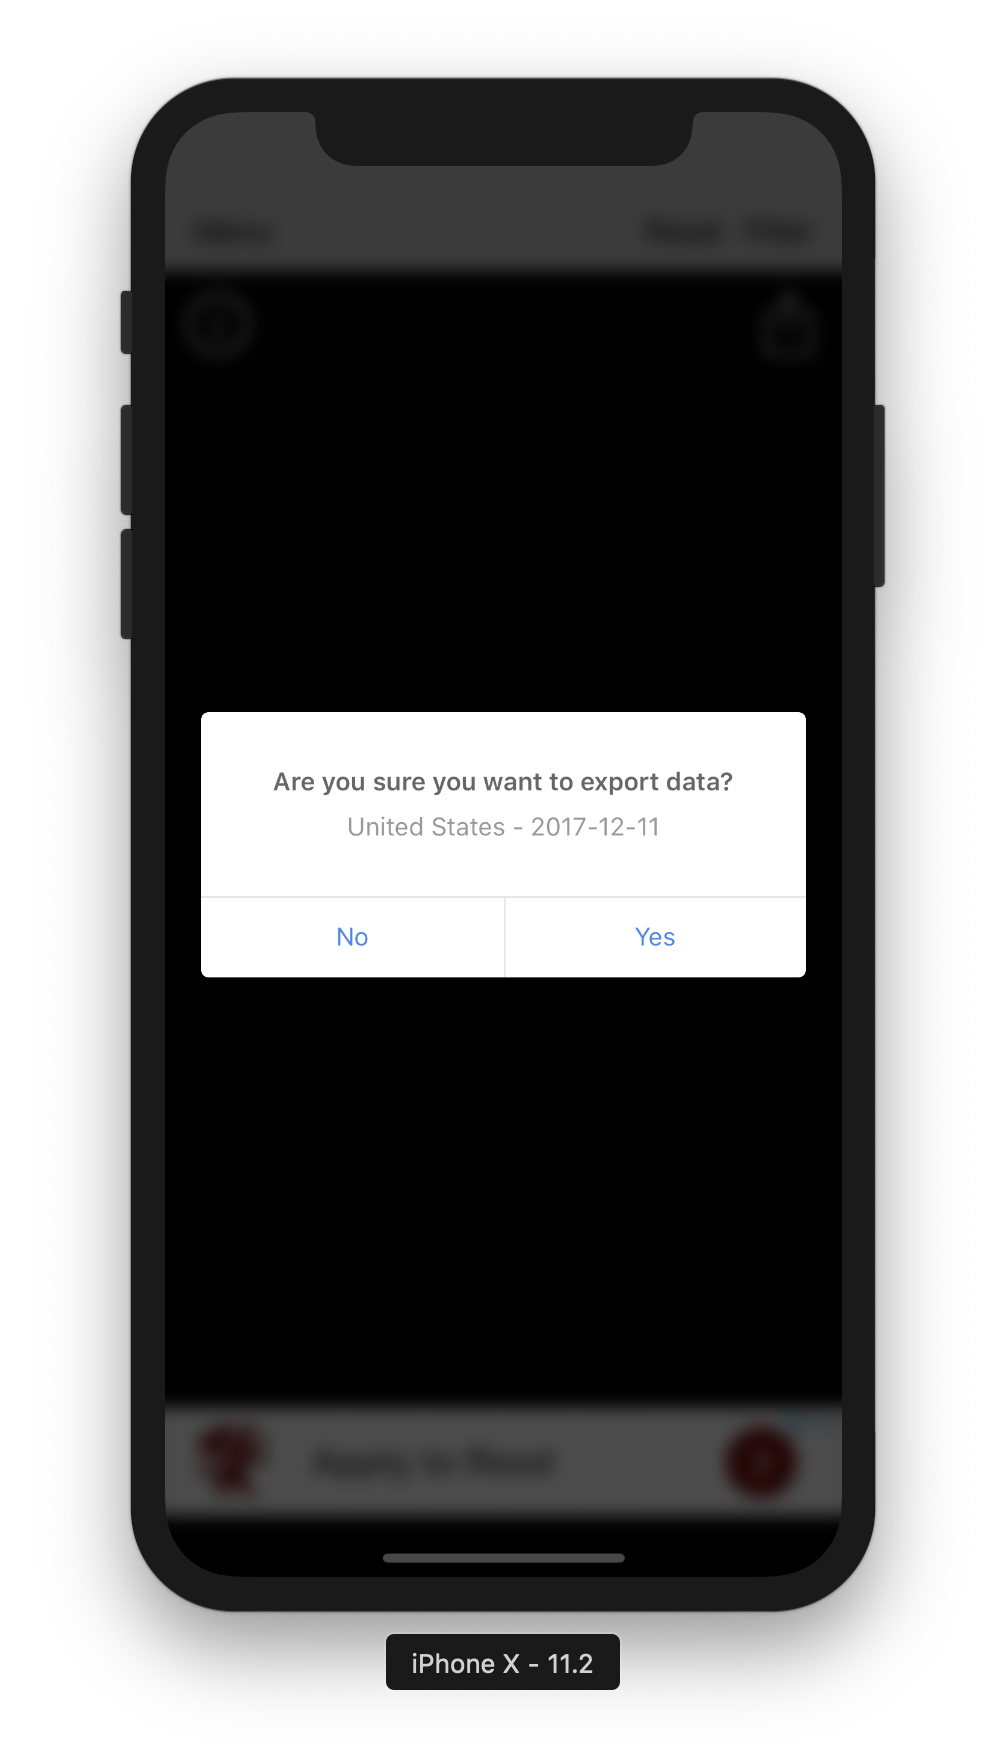
\includegraphics[width=0.25\linewidth]{figures/ch5/export_view.png}
            \caption{\label{fig:export_button} Export button action on home screen}
    \end{figure}
    
    On selecting yes in figure 5.3, \gls{json} data is converted to a valid \gls{csv} format and attached as a file on the MFMailComposeViewController. According to Apple, It's a standard interface for managing, editing, and sending an email message in \gls{iOS} app. \cite{MFMailComposer} Figure 5.4 shows the MFMailComposerViewController view which helps user to email the \gls{csv} file. 
    
    \begin{figure}[H]
            \centering
            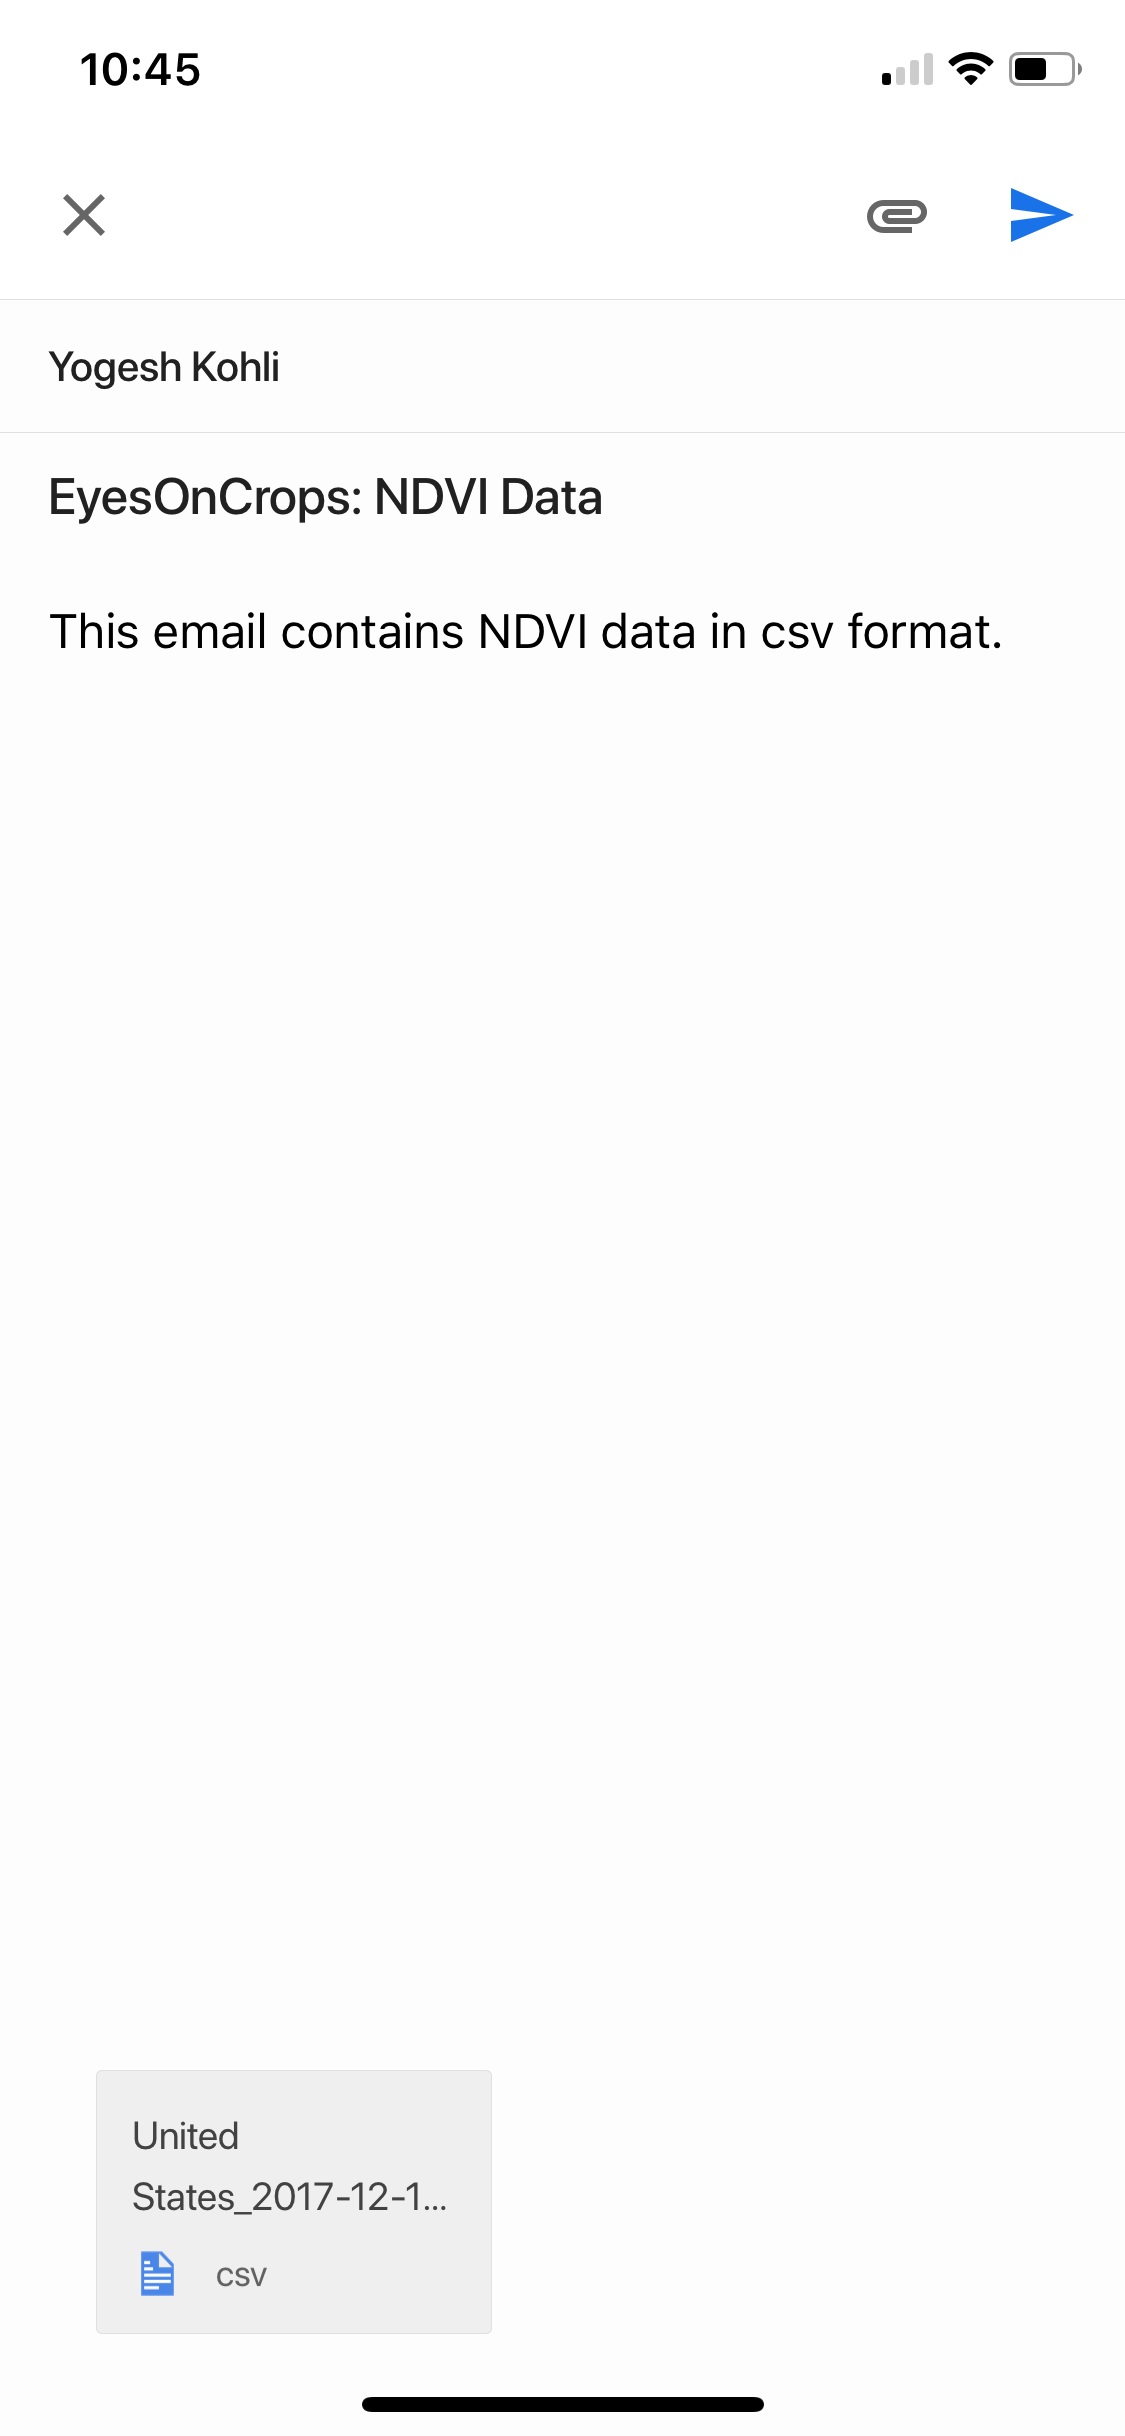
\includegraphics[width=0.25\linewidth]{figures/ch5/mfmailcomposer.png}
            \caption{\label{fig:email_controller} Email controller after selecting yes on export action screen}
    \end{figure}
    
\end{itemize}

\newpage

\section{Computing mean, standard deviation and histogram}

\begin{itemize}
    \item \textbf{Mean} \\
    According to a paper published in 1997, the mean of a data set is simply the arithmetic average of the values in the set, obtained by summing the values and dividing by the number of values. Recall that when we summarize a data set in a frequency distribution, we are approximating the data set by "rounding" each value in a given class to the class mark. With this in mind, it is natural to define the mean of a frequency distribution by figure 5.5. \cite{Mean_SD}
    
    \begin{equation} \label{eq:mean_formula}
       \mu = \frac{1}{n} \sum\limits_{i=1}^{n}f_{i}x_{i} \doteq \sum\limits_{i=1}^{n}p_{i}x_{i}
    \end{equation}
    
    \item \textbf{Standard Deviation} \\
   It is defined as the amount computed to show the degree of deviation for a gathering all in all.
   
  \begin{equation} \label{eq:standarddeviation_formula}
      \sigma = \sqrt{\frac{\sum\limits_{i=1}^{n}(x_{i} - \mu)^2}{n}}
    \end{equation}
    

where $\sigma$ represents the standard deviation, $x_{i}$ are the individual values and $\mu$ represents the mean which can be calculated by equation 5.1.
    
\end{itemize}

\centerline{\textbf{Why use mean and standard deviation for analysis?}}

The main purpose of using mean and standard deviation as a parameter for analysis is that the Normal Curve discloses to us that numerical data will be disseminated in an pattern around a normal line whereas Standard deviation is viewed as the most valuable list of variability. It is a solitary number that discloses to us the inconstancy, or spread, of an appropriation (gathering of scores). We have investigated \gls{ndvi} and Anomaly a portion of the nations just to demonstrate that with the sent out information through the app, client can do these things:

\newpage

\begin{itemize}
    \item \textbf{Mean NDVI \& Anomaly distribution over the years}
    
     \begin{figure}[H]
            \centering
            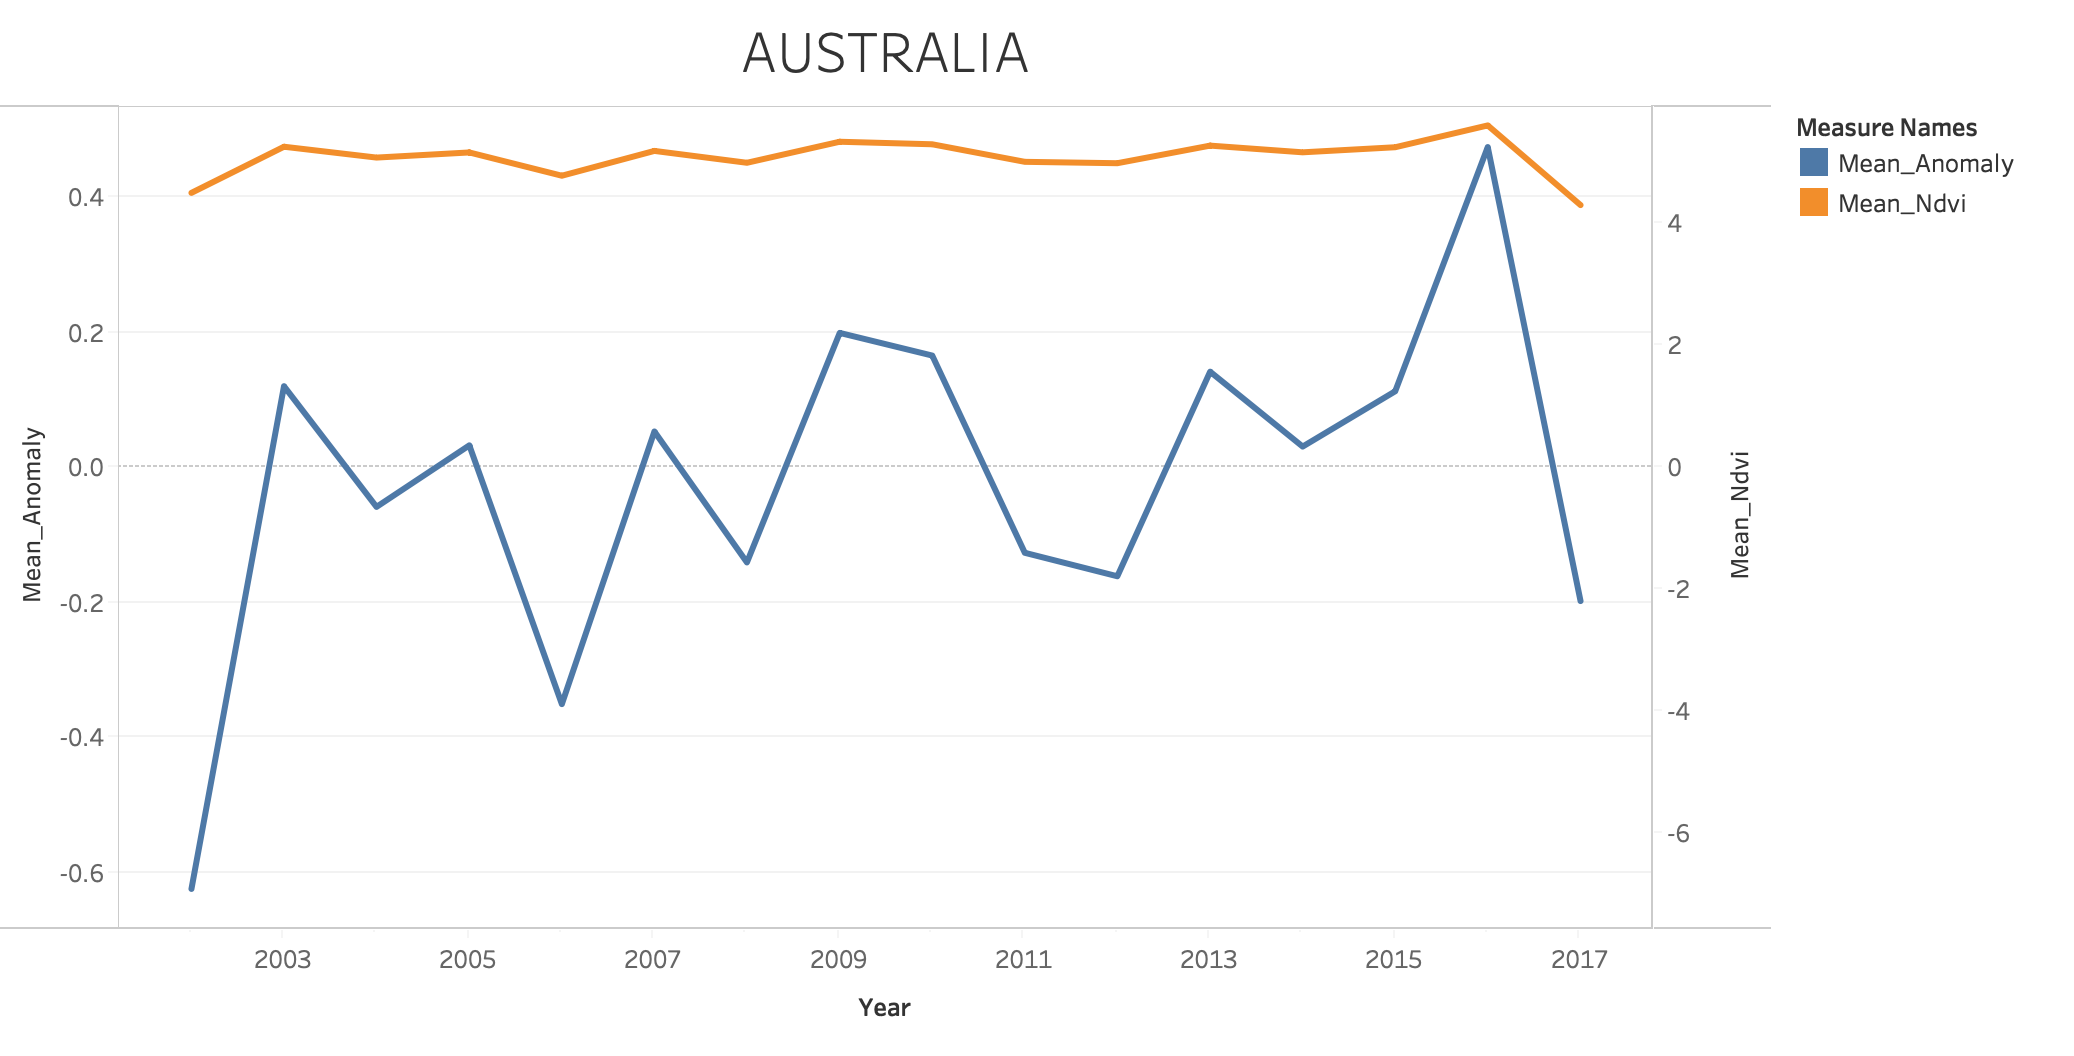
\includegraphics[width=1.0\linewidth]{figures/ch5/Mean/AUSTRALIA_mean.png}
            \caption{Mean graph - Australia}\label{Fig:AUSTRALIA_mean}
    \end{figure}
    
    \begin{figure}[H]
            \centering
            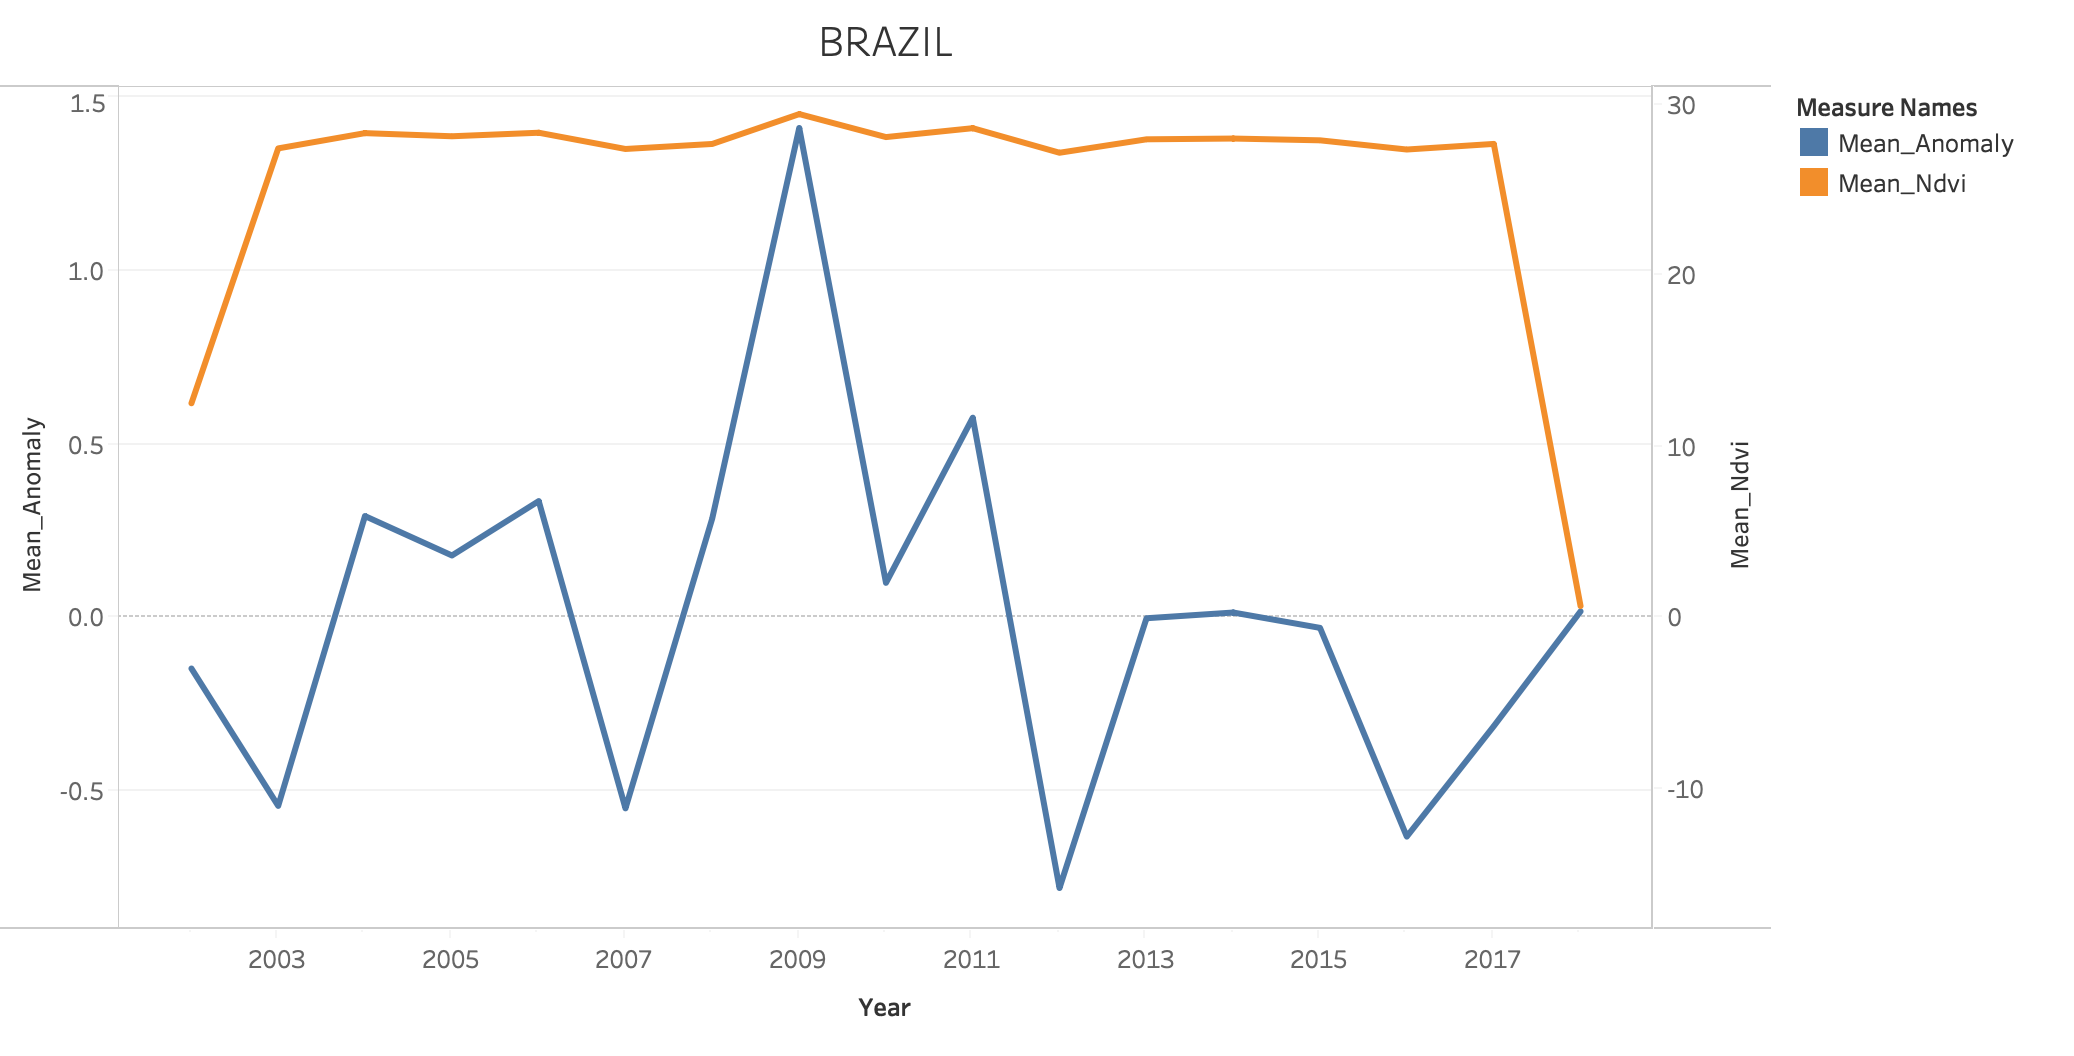
\includegraphics[width=1.0\linewidth]{figures/ch5/Mean/BRAZIL_mean.png}
            \caption{Mean graph - Brazil}\label{Fig:BRAZIL_mean}
    \end{figure}
    
    \begin{figure}[H]
            \centering
            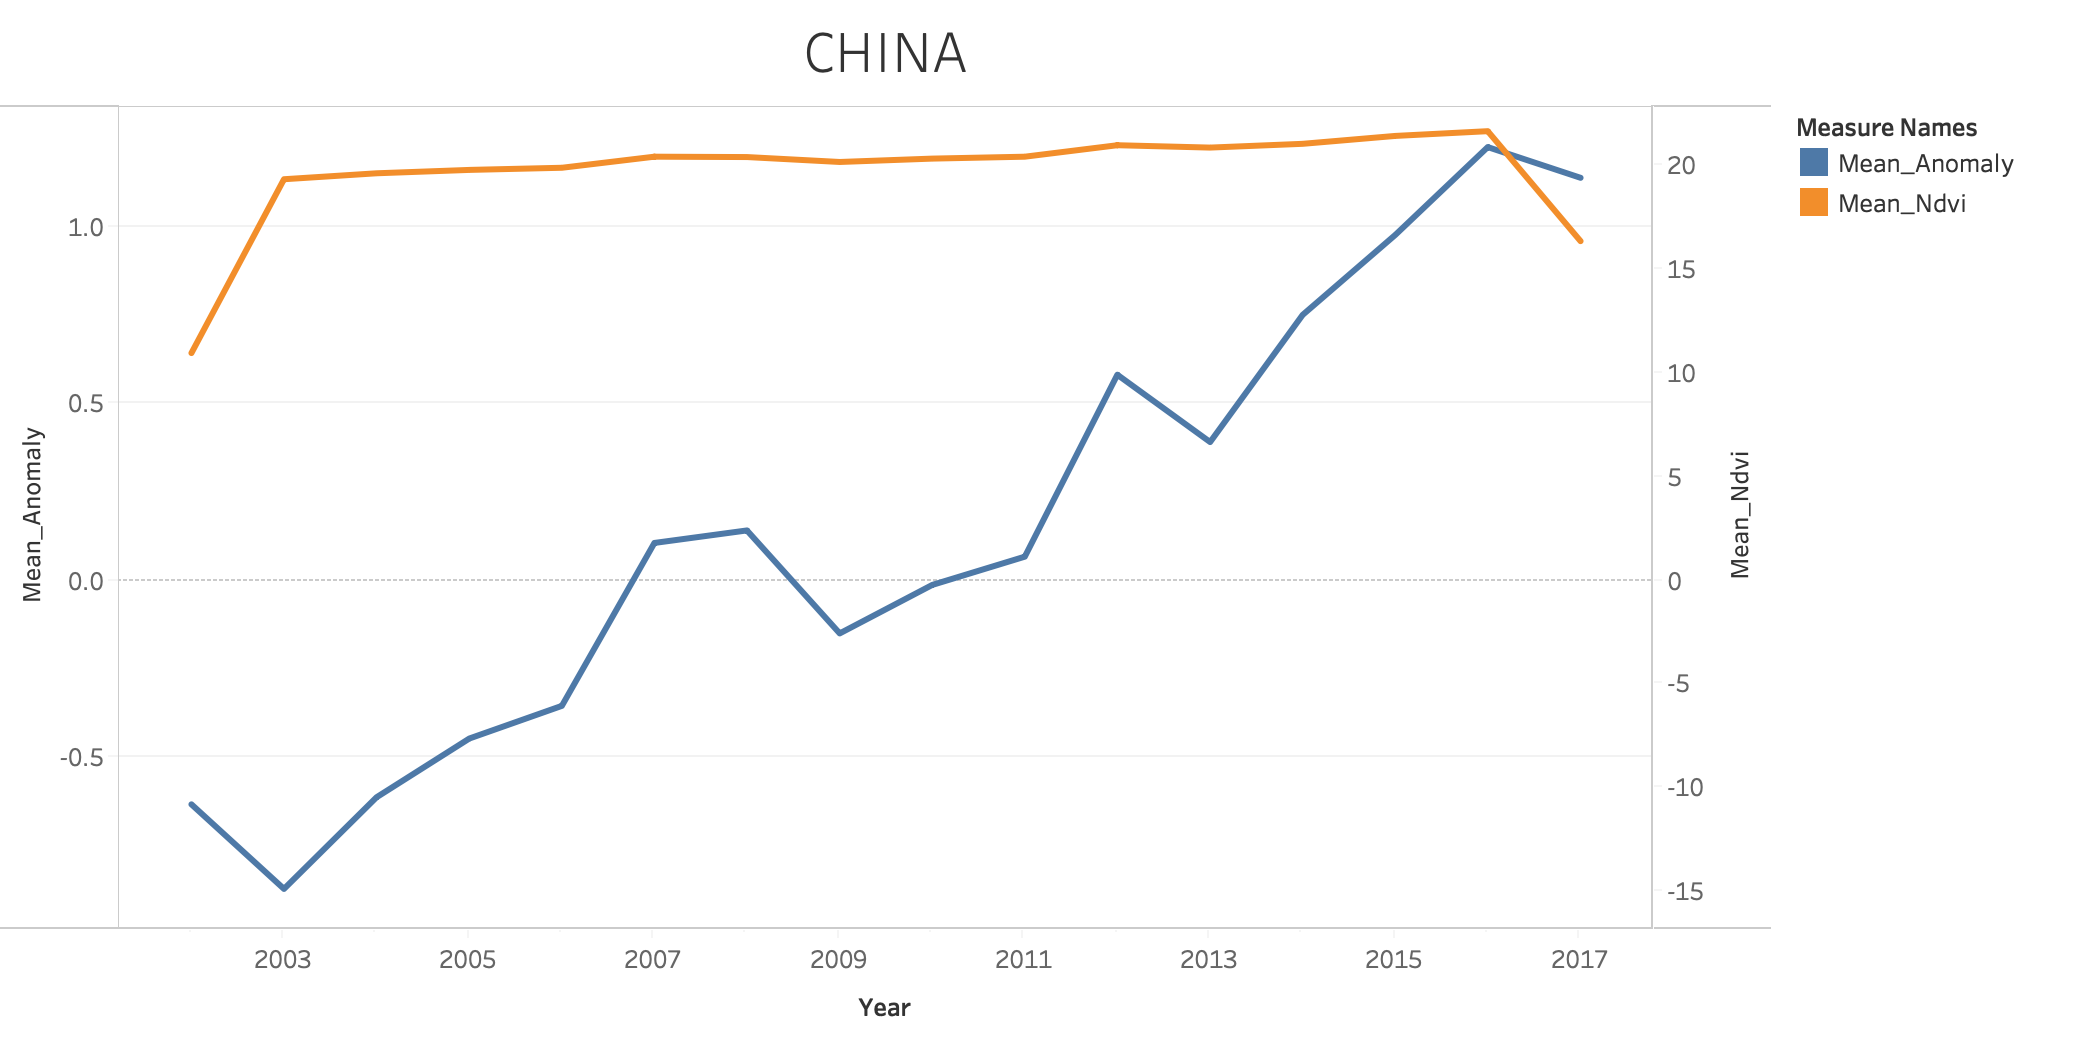
\includegraphics[width=1.0\linewidth]{figures/ch5/Mean/CHINA_mean.png}
            \caption{Mean graph - China}\label{Fig:CHINA_mean}
    \end{figure}
    
    \begin{figure}[H]
            \centering
            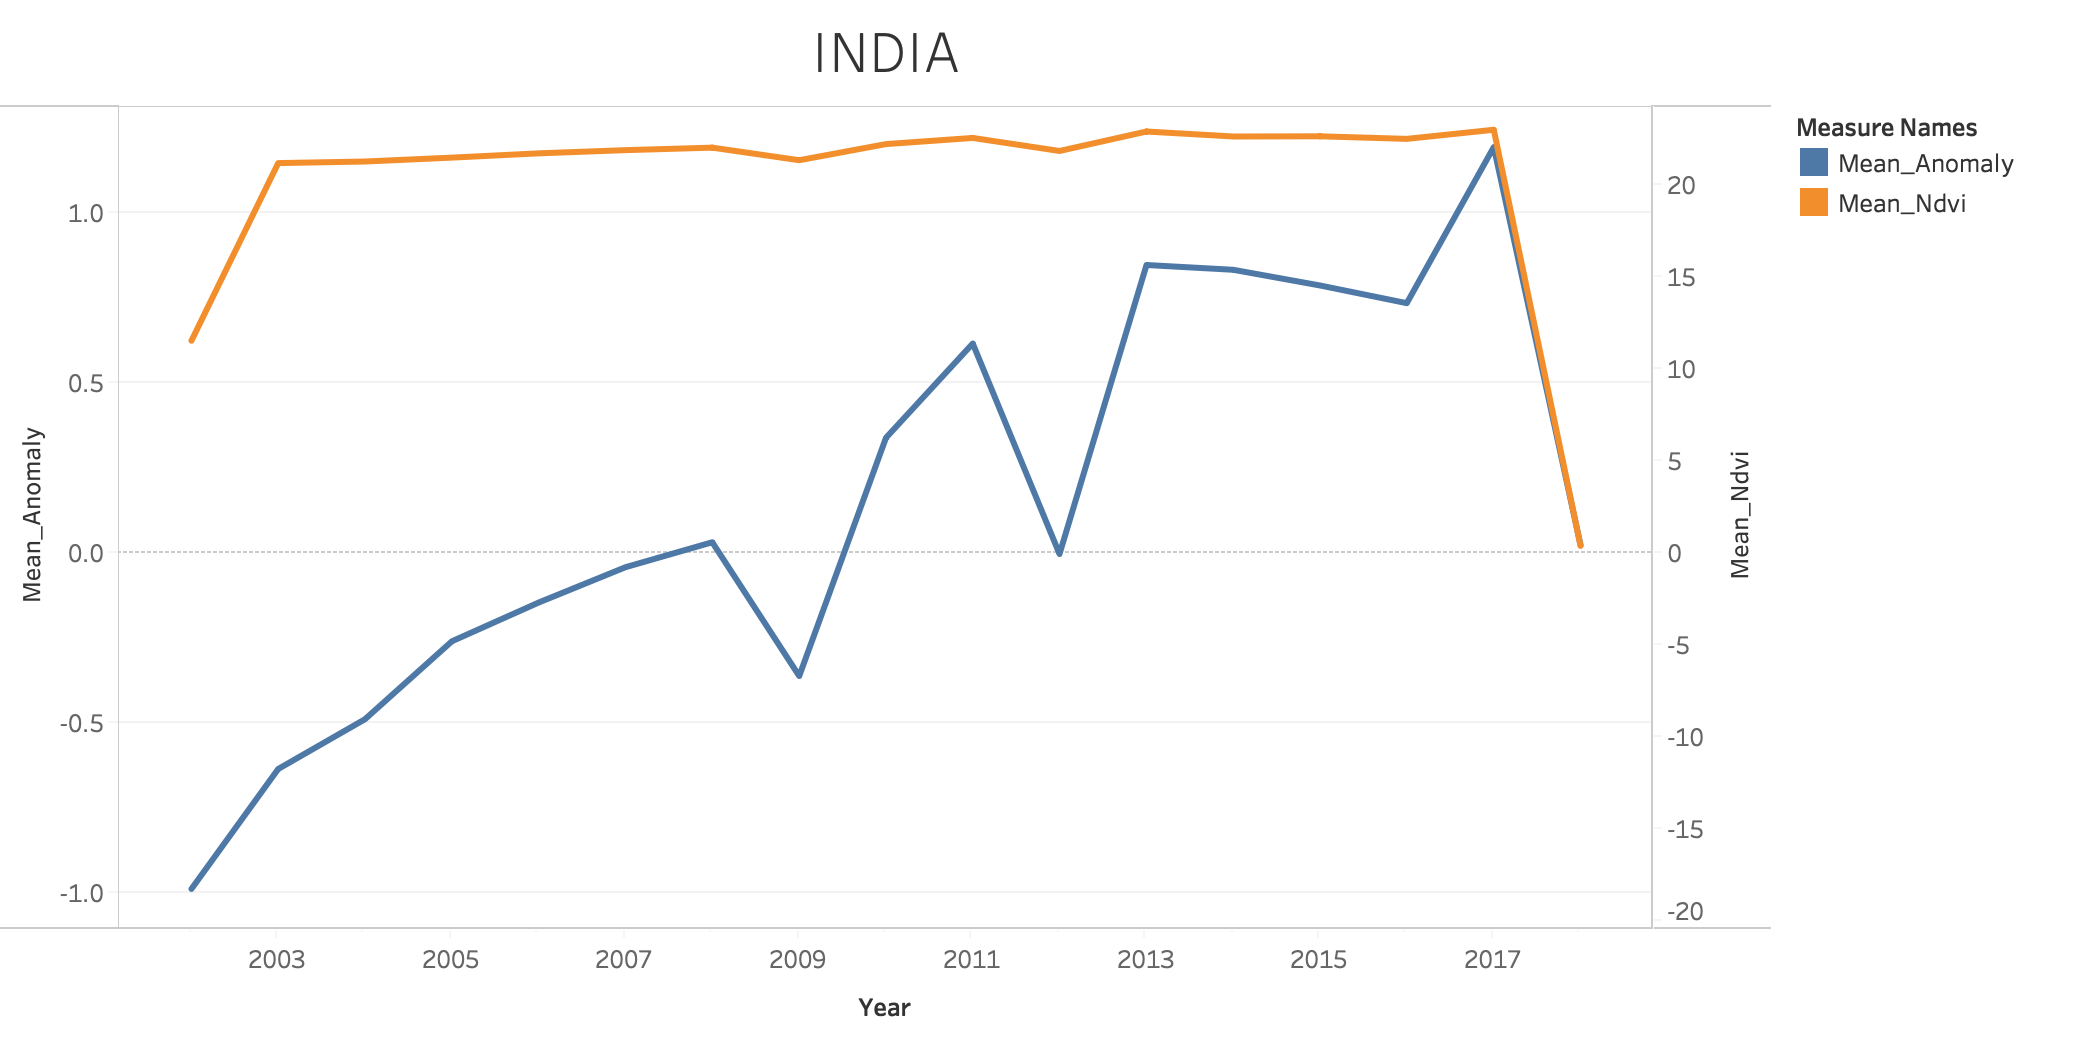
\includegraphics[width=1.0\linewidth]{figures/ch5/Mean/INDIA_mean.png}
            \caption{Mean graph - India}\label{Fig:INDIA_mean}
    \end{figure}
    
     \begin{figure}[H]
            \centering
            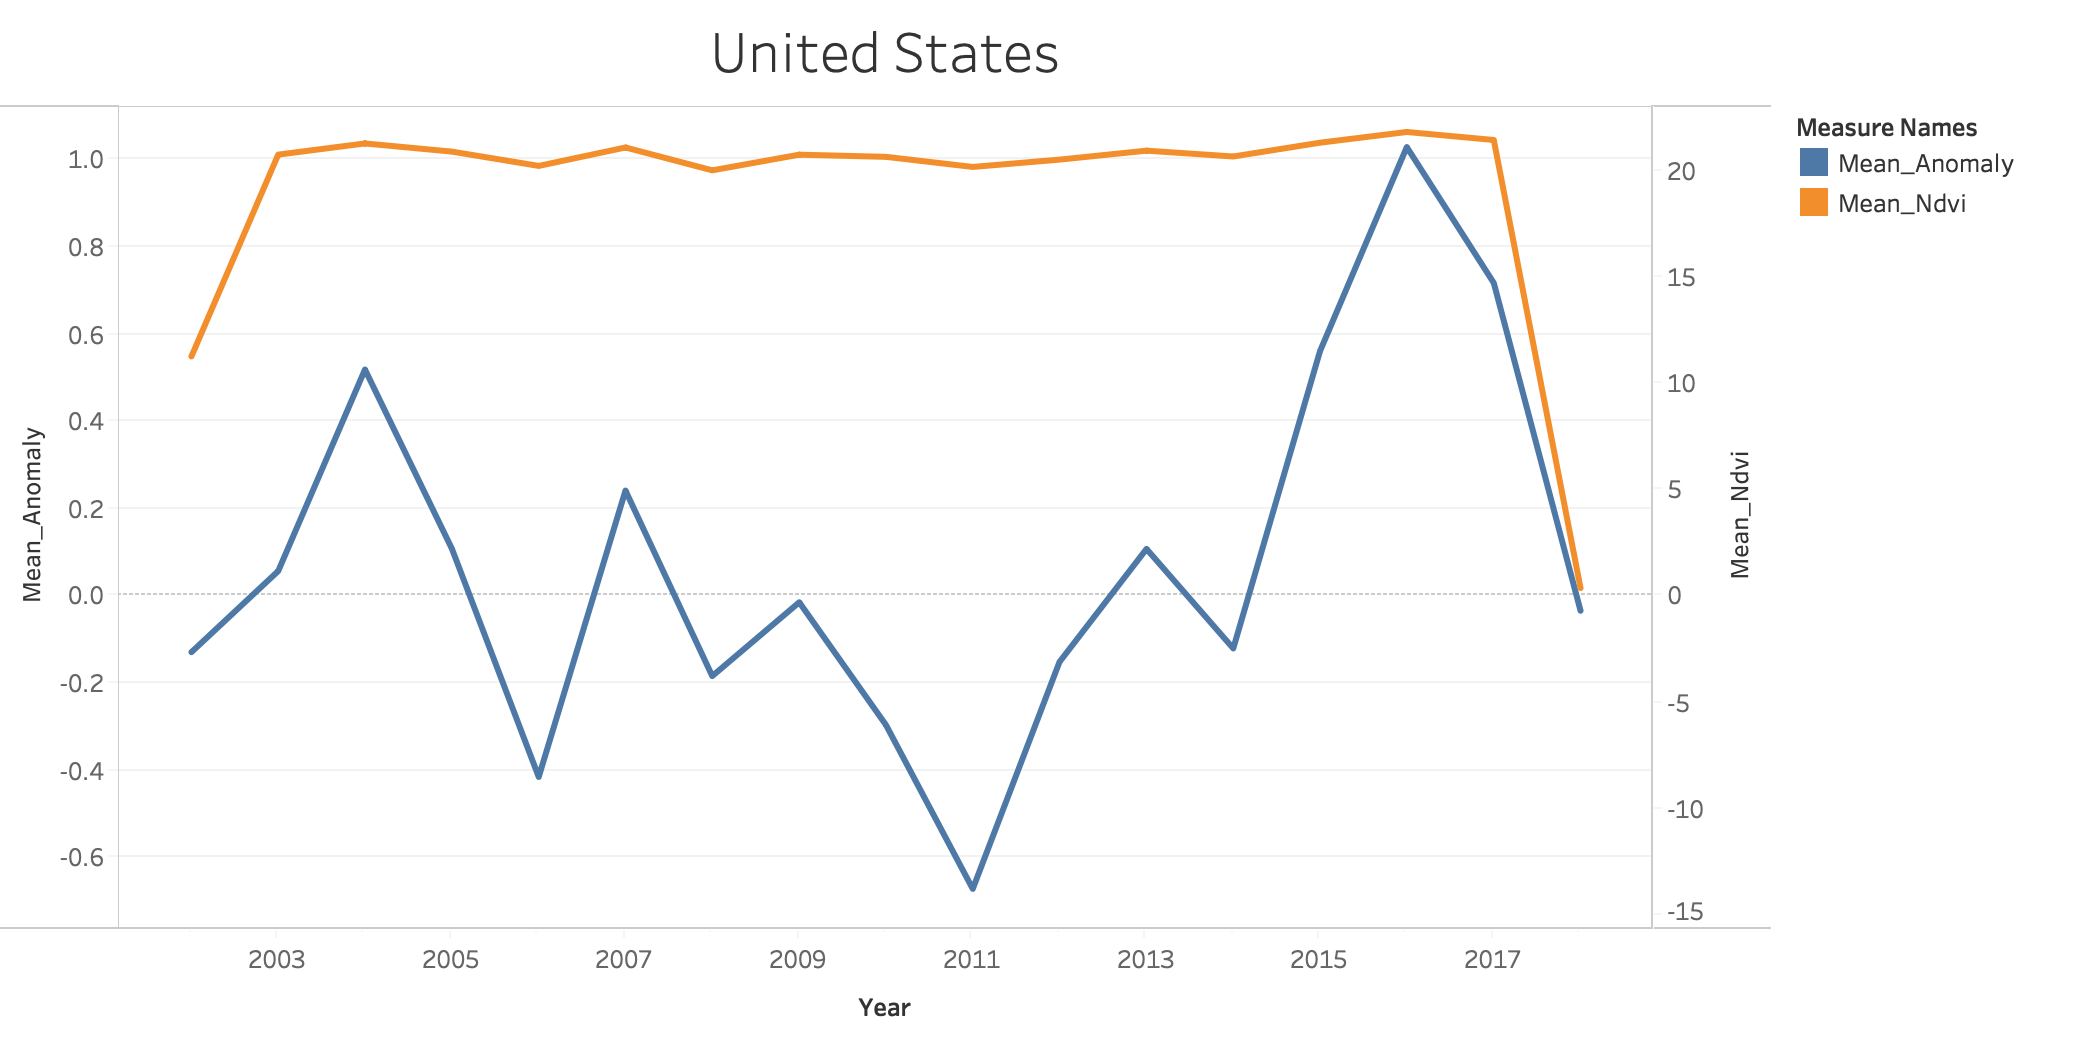
\includegraphics[width=1.0\linewidth]{figures/ch5/Mean/US_mean.png}
            \caption{\label{fig:US_mean}Mean graph - United States}
    \end{figure}

    \item \textbf{Standard Deviation NDVI \& Anomaly distribution over the years}
    
    \begin{figure}[H]
            \centering
            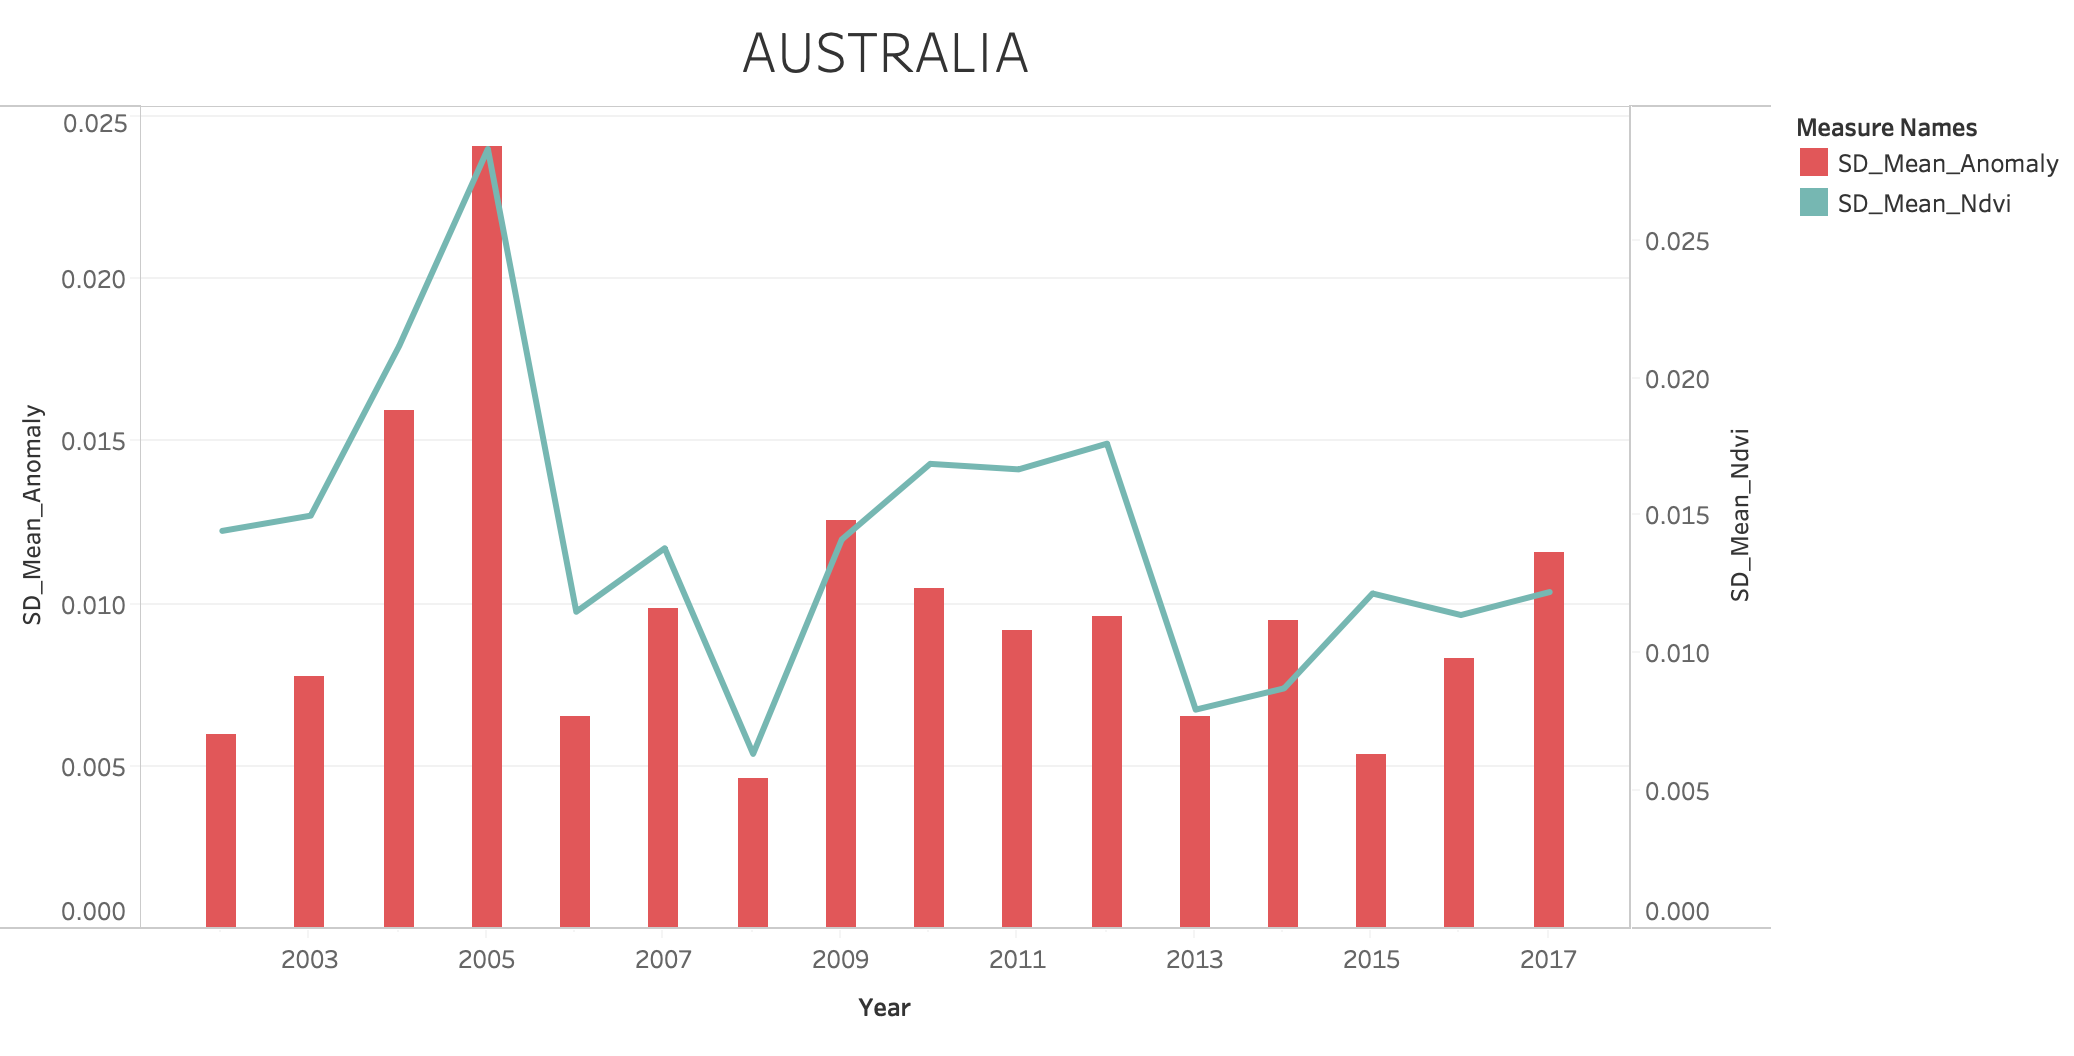
\includegraphics[width=1.0\linewidth]{figures/ch5/StandardDeviation/AUSTRALIA_SD.png}
            \caption{Standard deviation graph - Australia}\label{Fig:AUSTRALIA_SD}
    \end{figure}
    
    \begin{figure}[H]
            \centering
             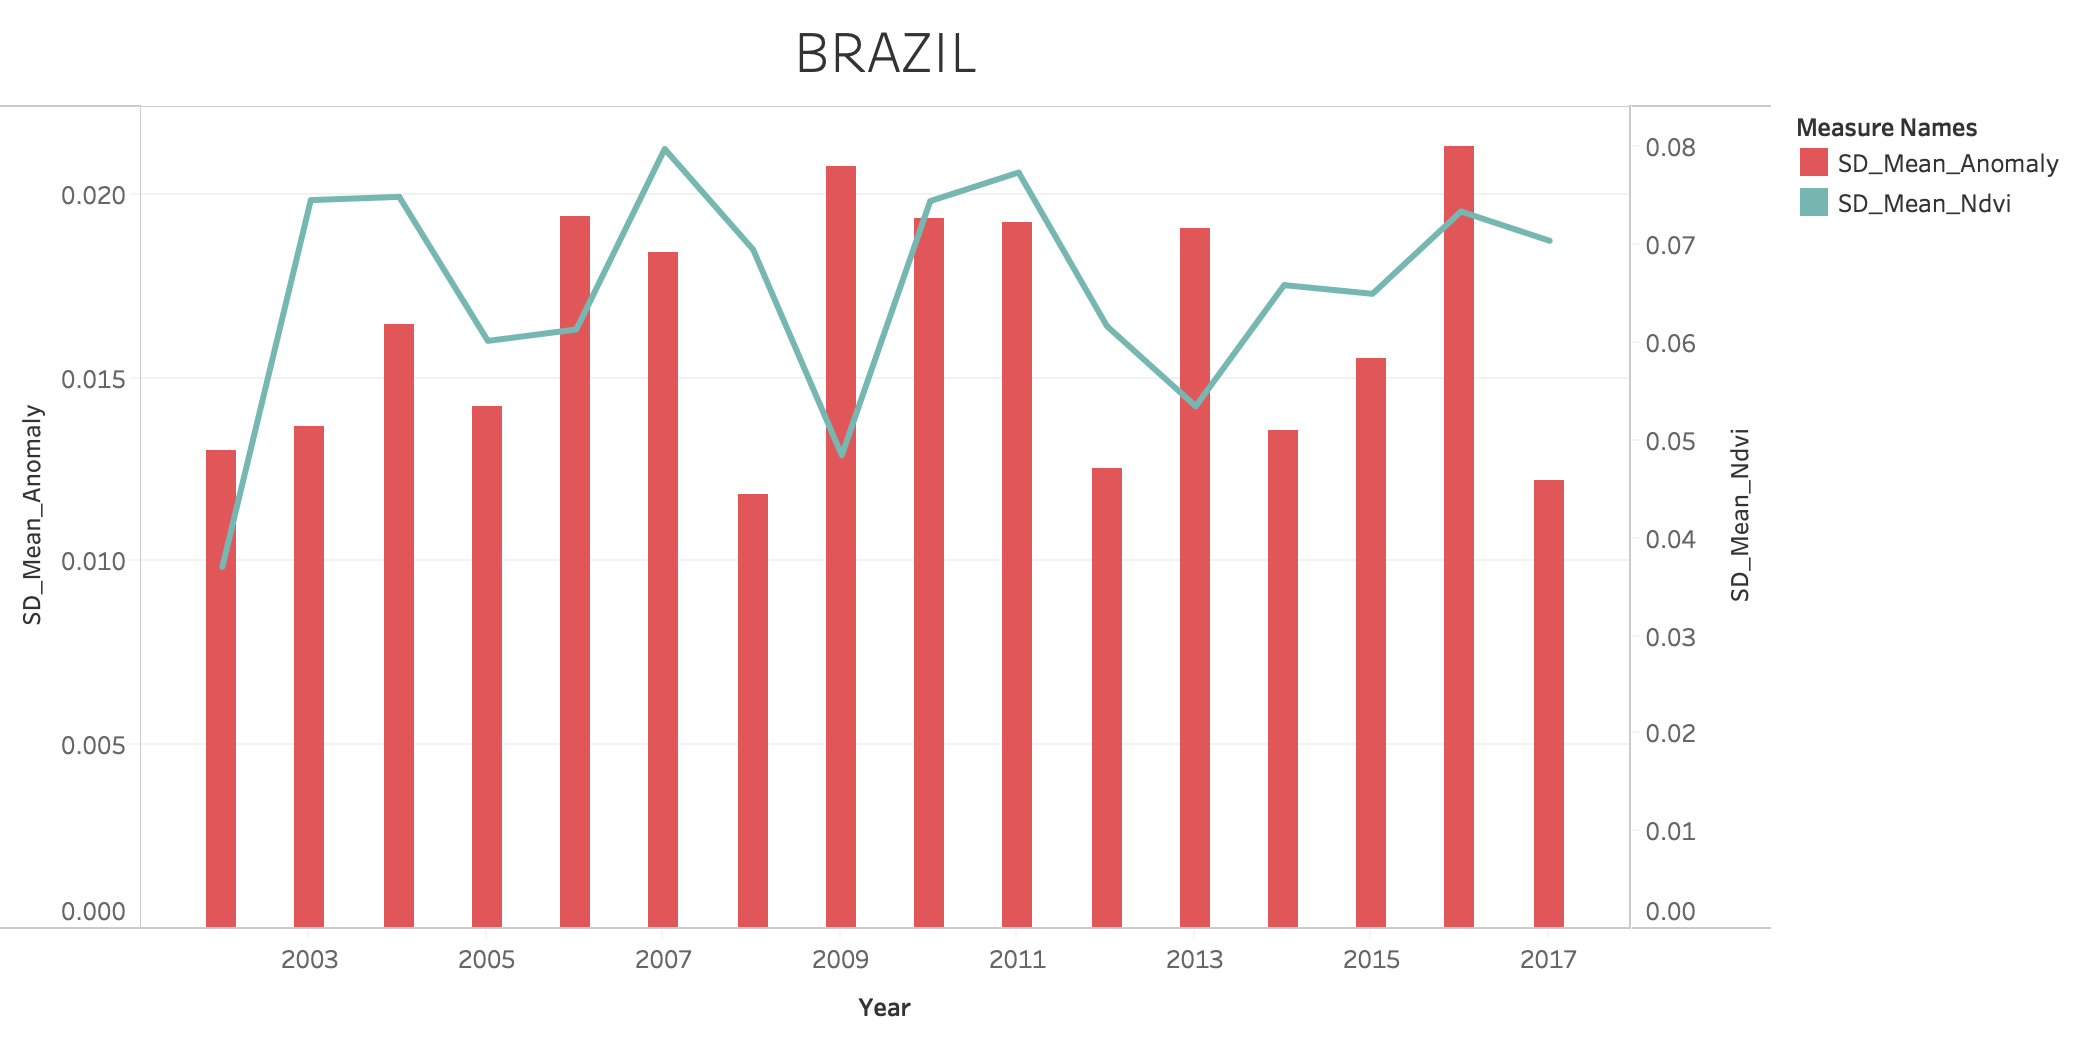
\includegraphics[width=1.0\linewidth]{figures/ch5/StandardDeviation/BRAZIL_SD.png}
            \caption{Standard deviation graph - Brazil}\label{Fig:BRAZIL_SD}
    \end{figure}
    
    \begin{figure}[H]
            \centering
            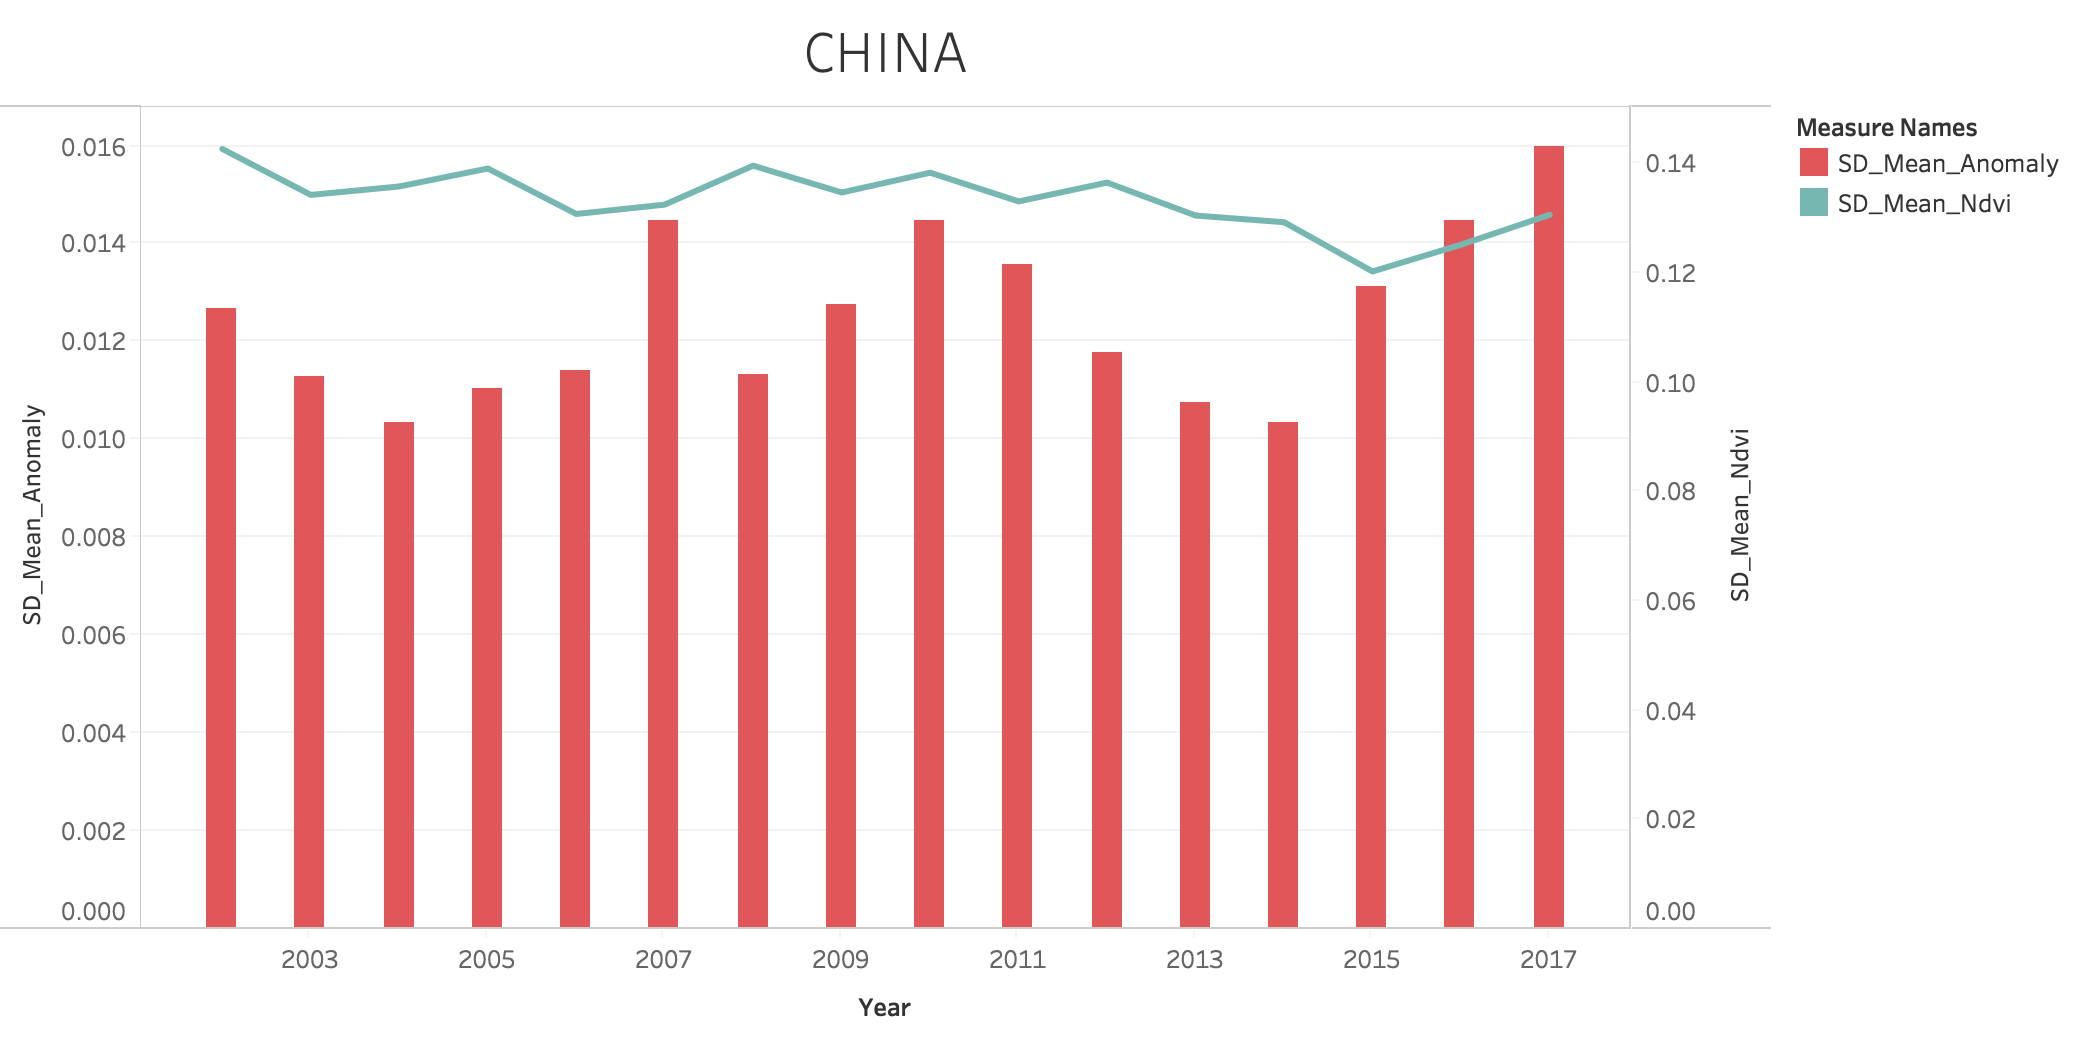
\includegraphics[width=1.0\linewidth]{figures/ch5/StandardDeviation/CHINA_SD.png}
            \caption{Standard deviation graph - China}\label{Fig:CHINA_SD}
    \end{figure}
    
    \begin{figure}[H]
            \centering
            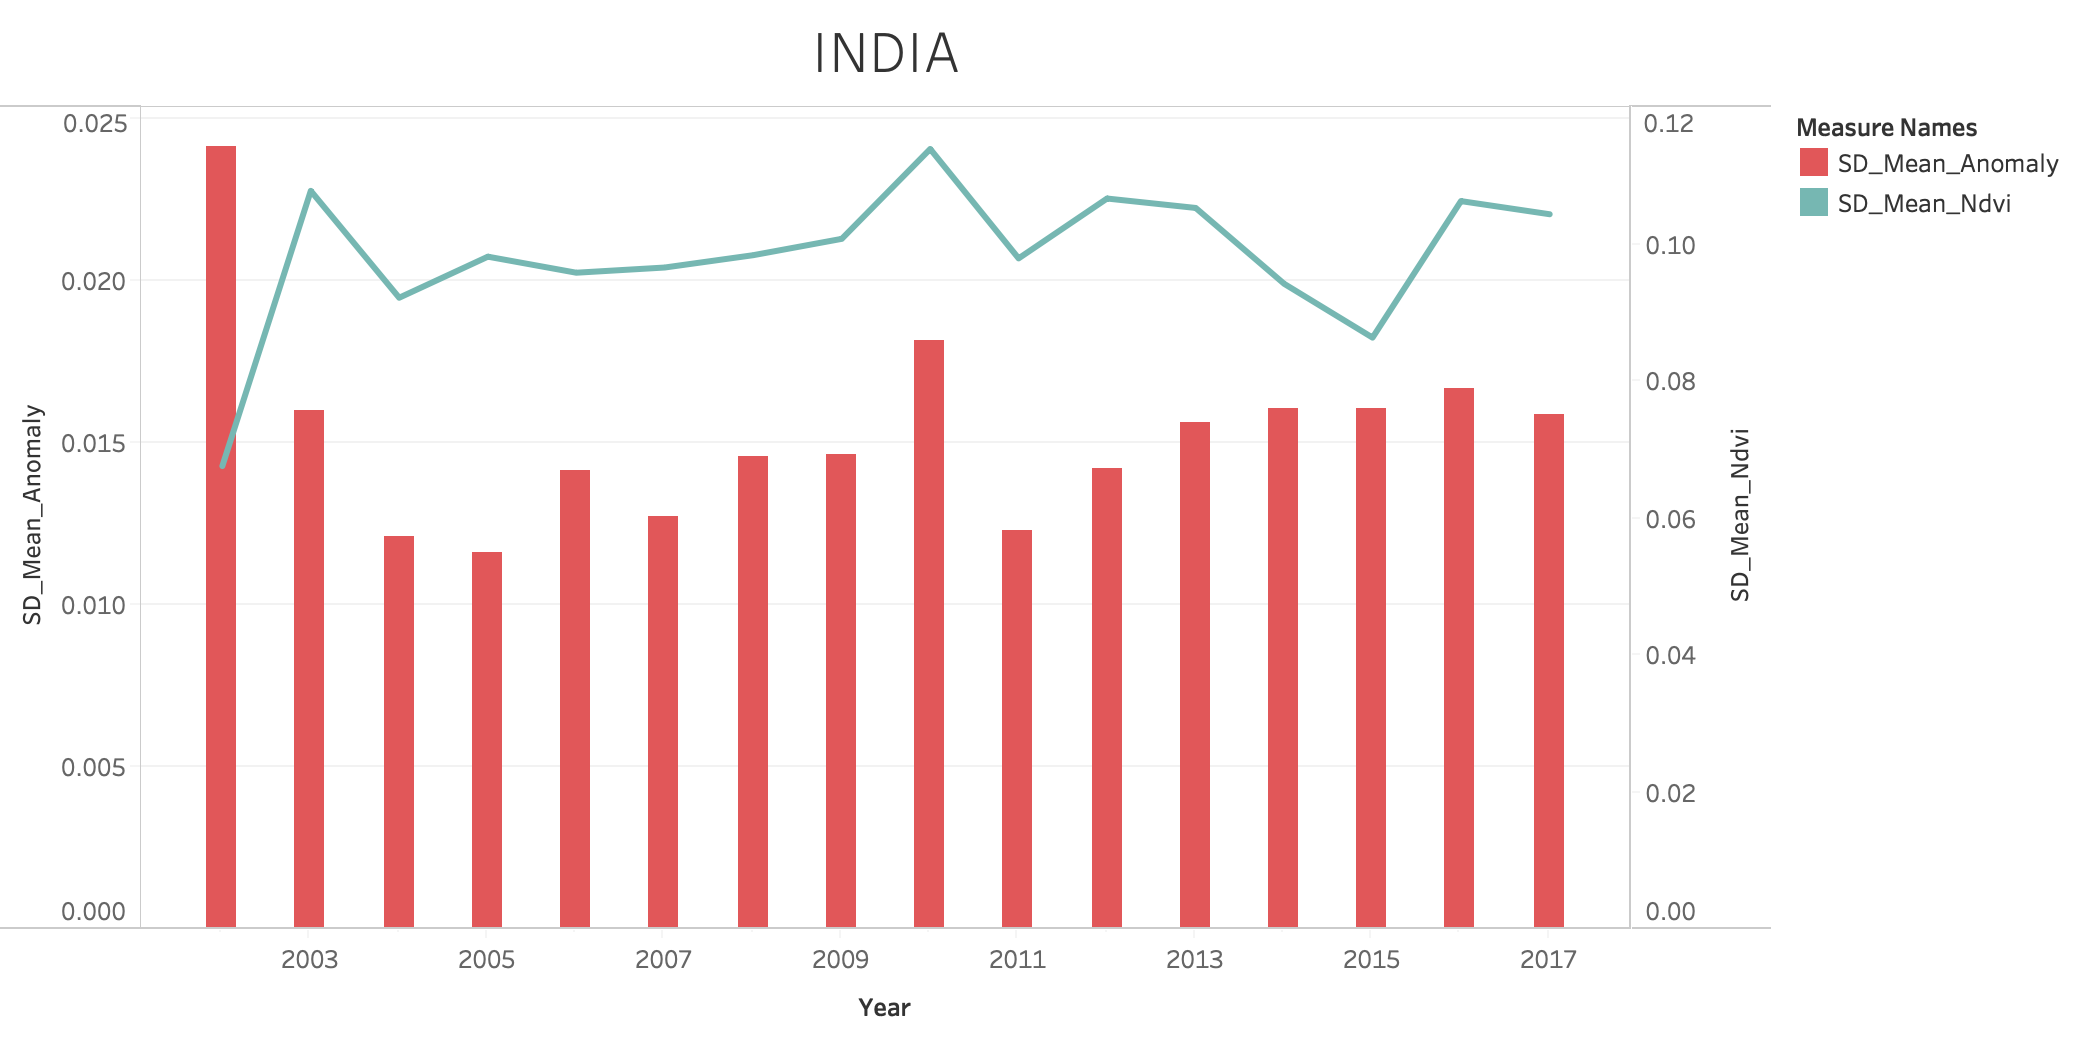
\includegraphics[width=1.0\linewidth]{figures/ch5/StandardDeviation/INDIA_SD.png}
            \caption{Standard deviation graph - India}\label{Fig:INDIA_SD}
    \end{figure}
    
     \begin{figure}[H]
            \centering
            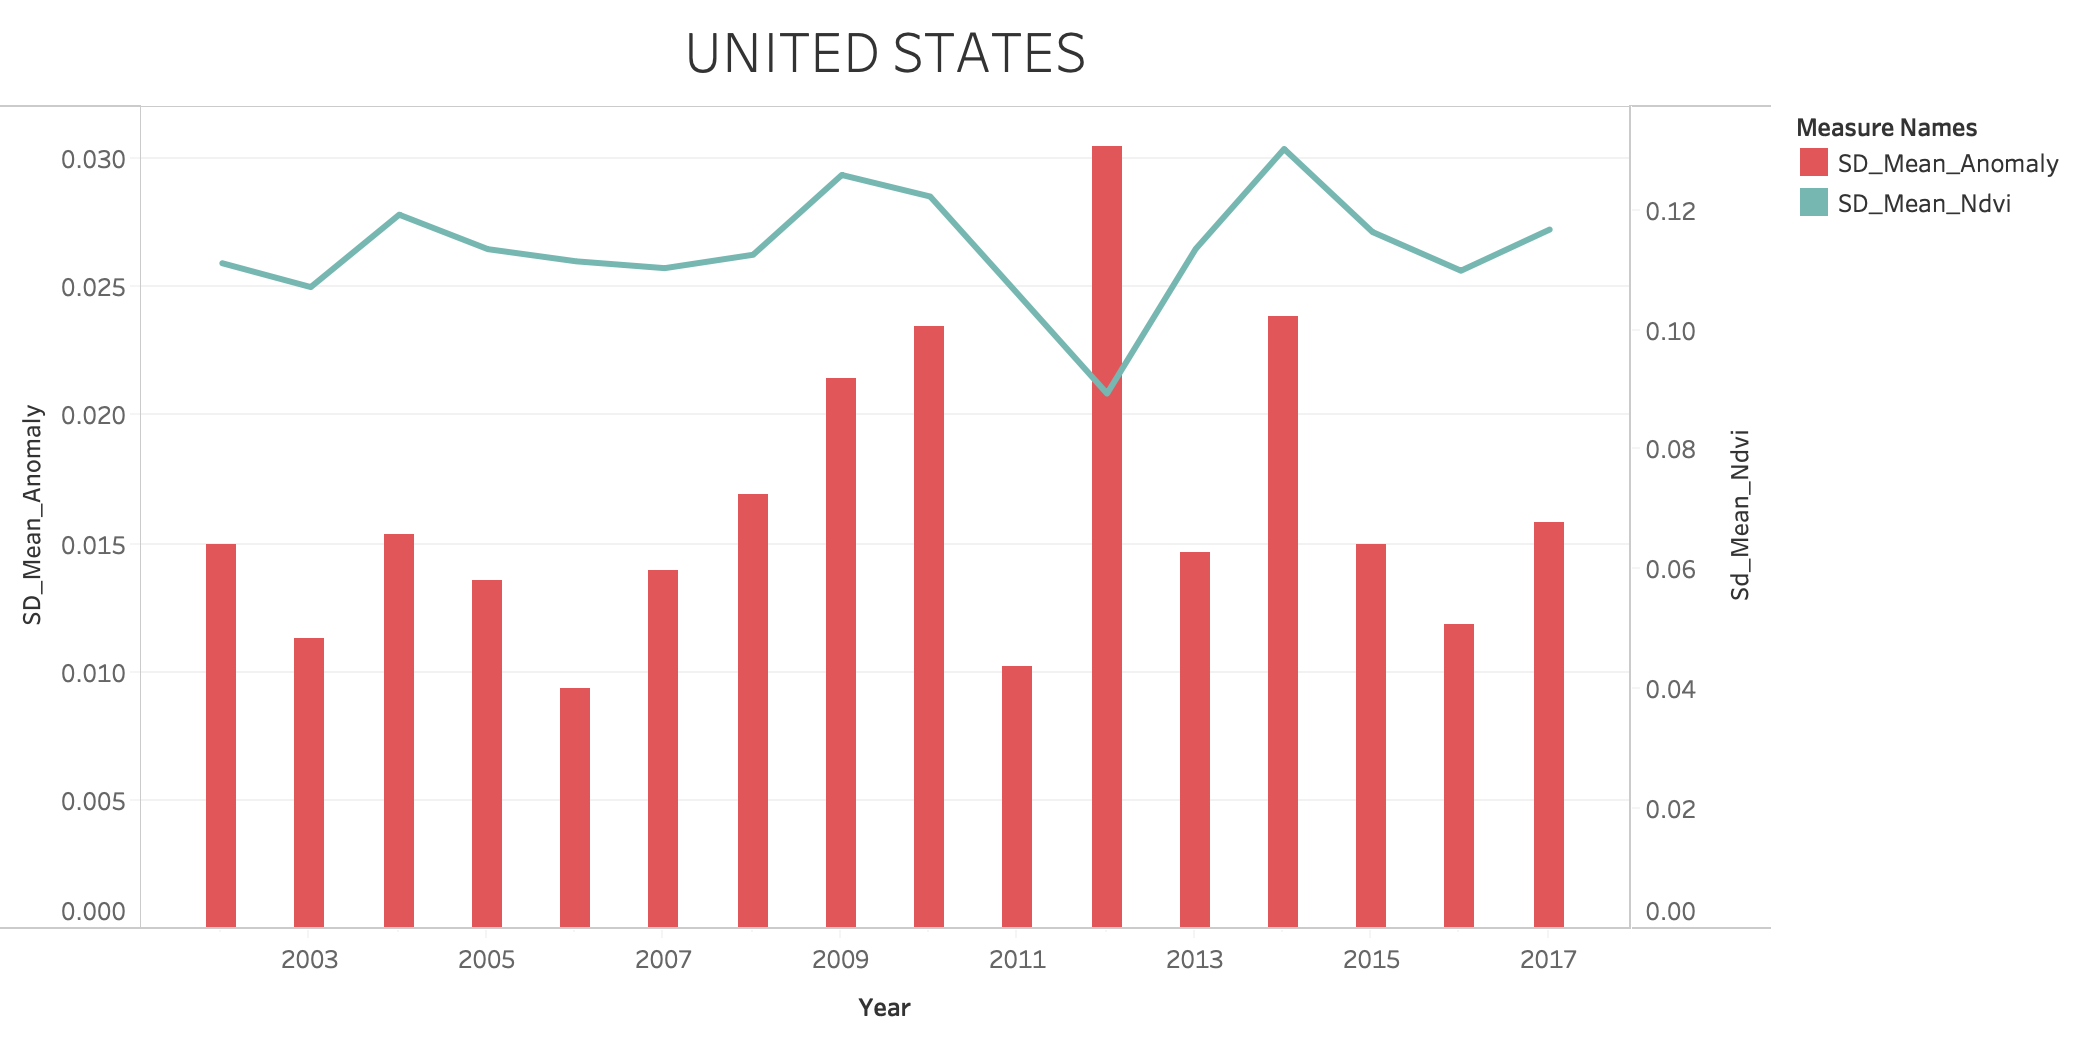
\includegraphics[width=1.0\linewidth]{figures/ch5/StandardDeviation/US_SD.png}
            \caption{\label{fig:US_SD}Standard deviation graph - United States}
    \end{figure}
   
    \newpage
    
    \item \textbf{Histogram NDVI \& Anomaly distribution over the years}
    
    \begin{figure}[H]
            \centering
            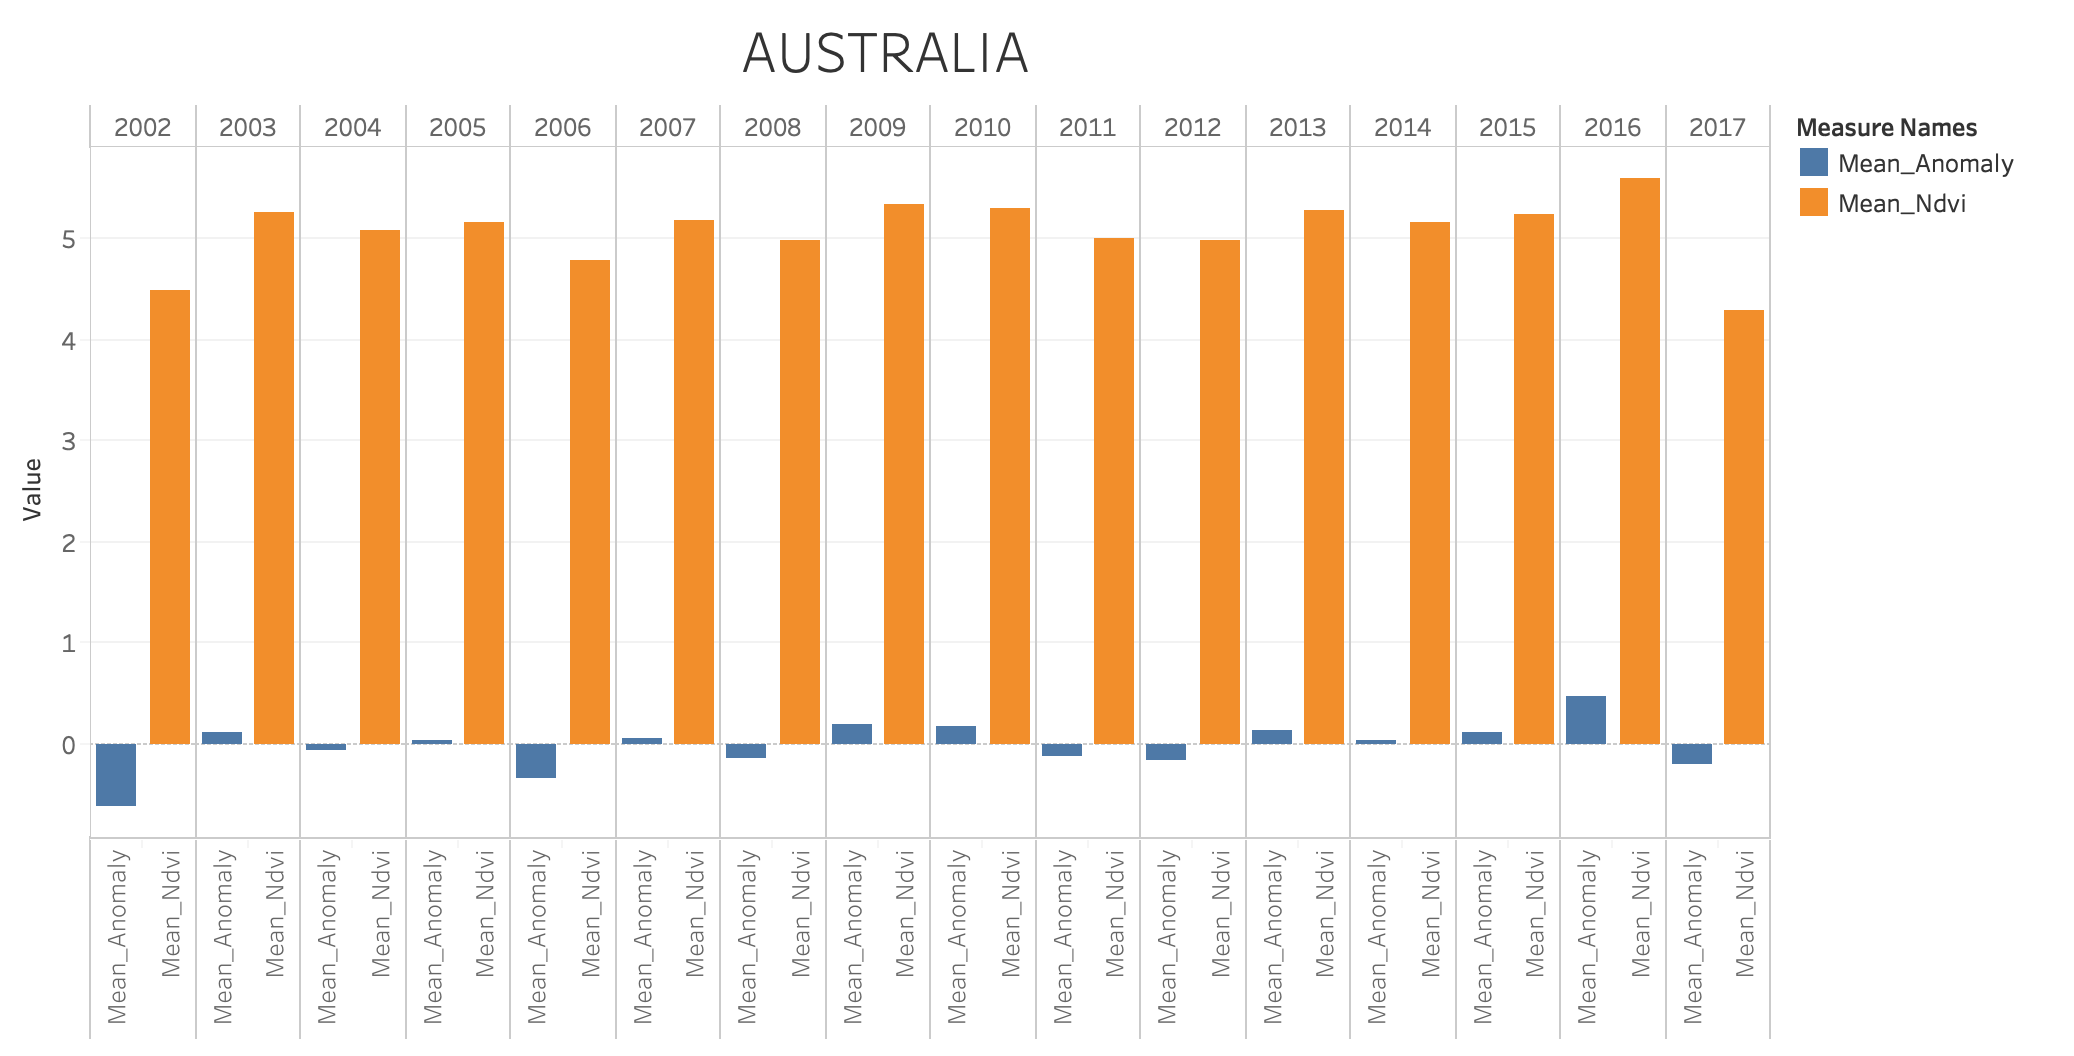
\includegraphics[width=1.0\linewidth]{figures/ch5/Histograms/AUSTRALIA_histogram.png}
            \caption{Histogram graph - Australia}\label{Fig:AUSTRALIA_histogram}
    \end{figure}
    
    \begin{figure}[H]
            \centering
            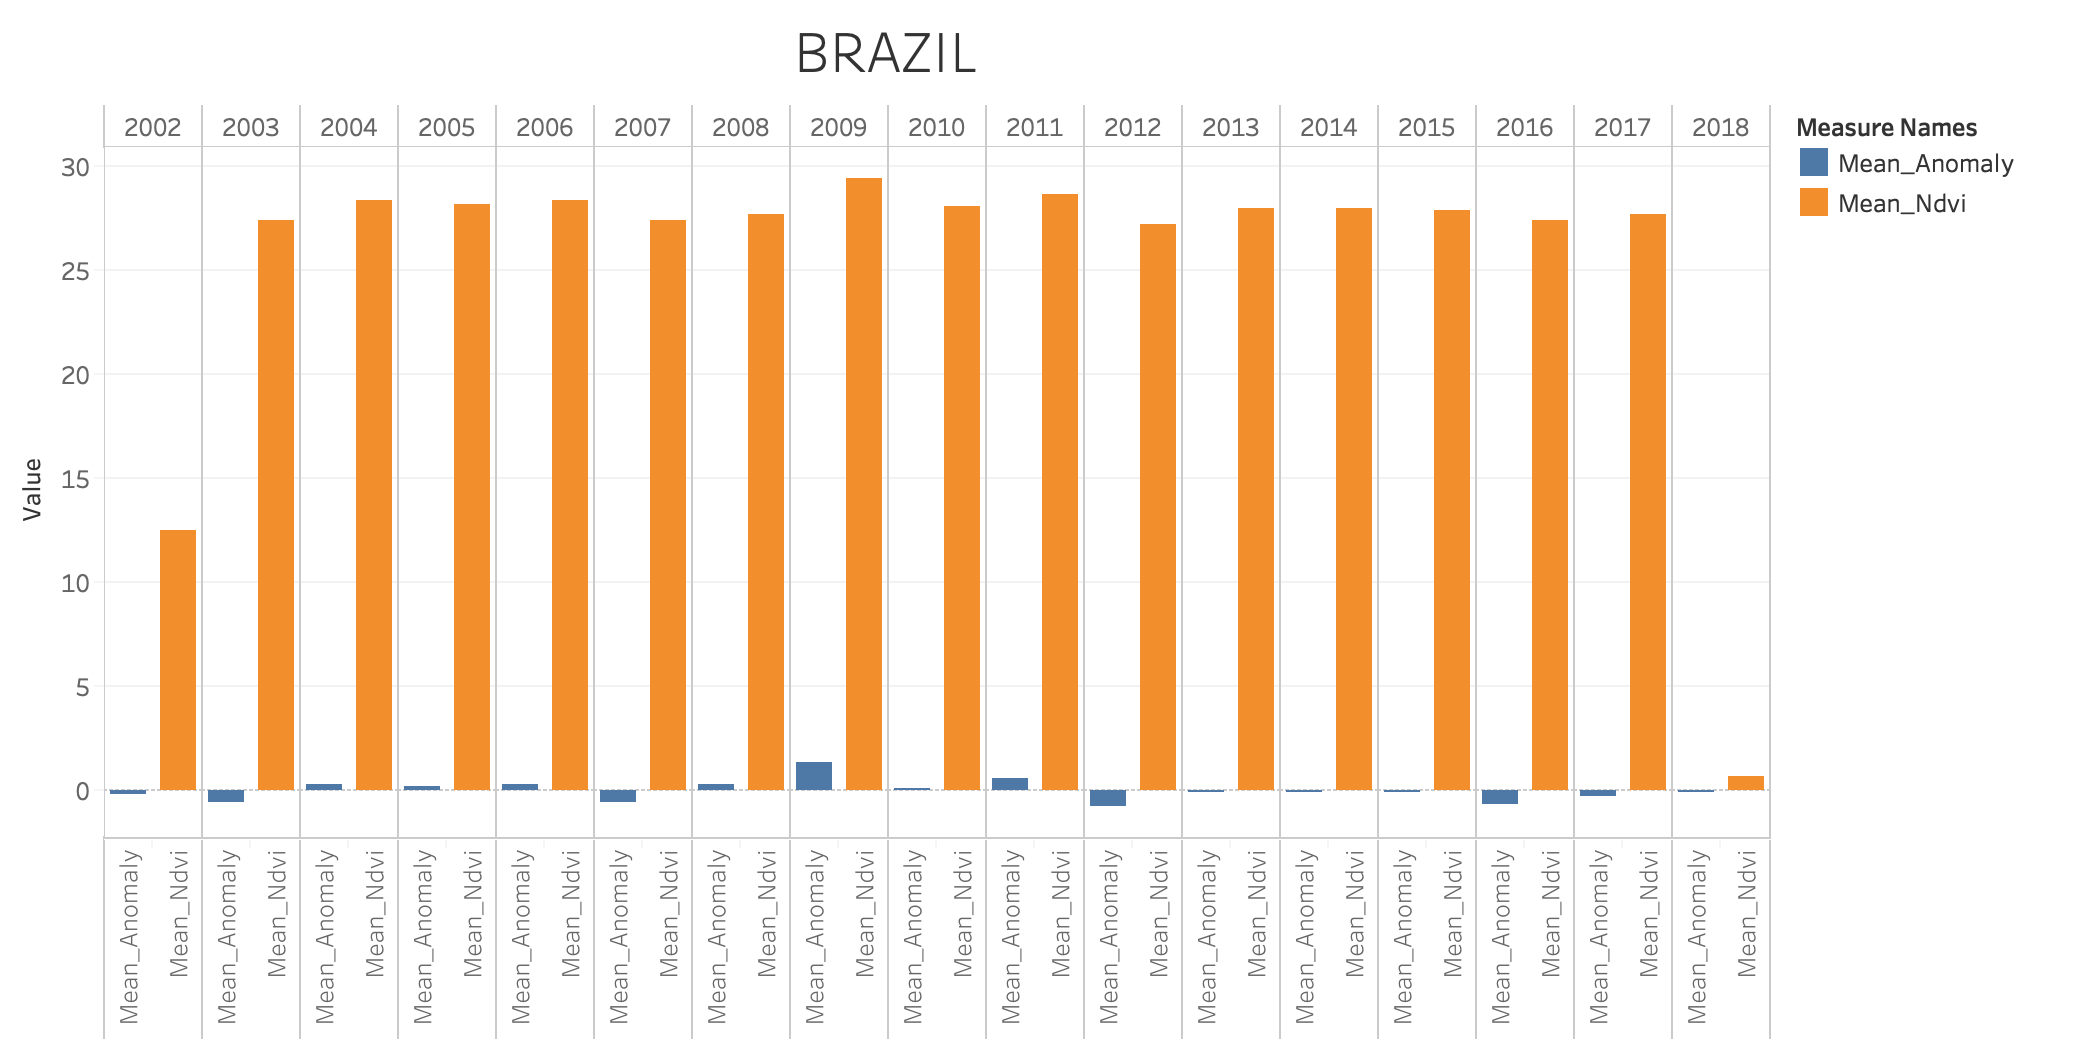
\includegraphics[width=1.0\linewidth]{figures/ch5/Histograms/BRAZIL_histogram.png}
            \caption{Histogram graph - Brazil}\label{Fig:BRAZIL_histogram}
    \end{figure}
    
    \begin{figure}[H]
            \centering
            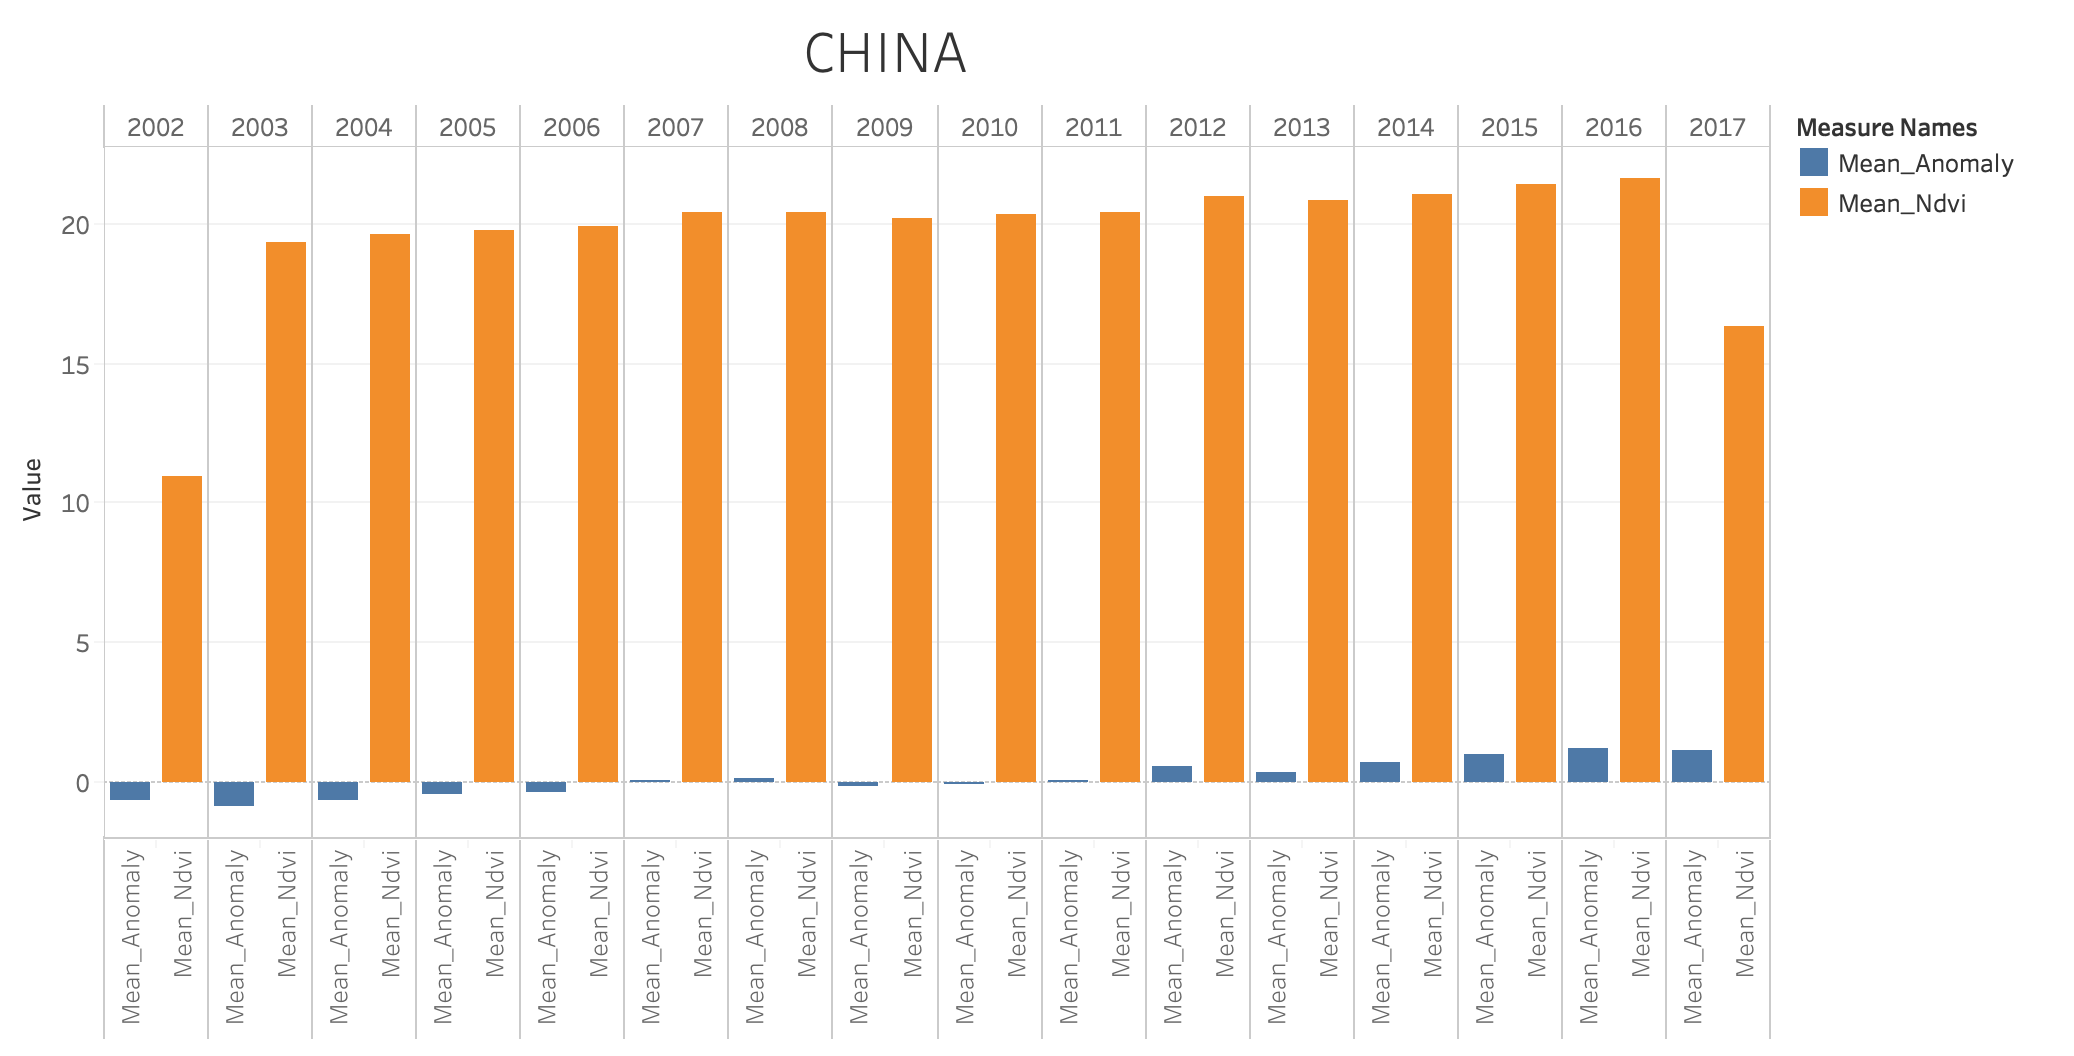
\includegraphics[width=1.0\linewidth]{figures/ch5/Histograms/CHINA_histogram.png}
            \caption{Histogram graph - China}\label{Fig:CHINA_histogram}
    \end{figure}
    
    
    \begin{figure}[H]
            \centering
            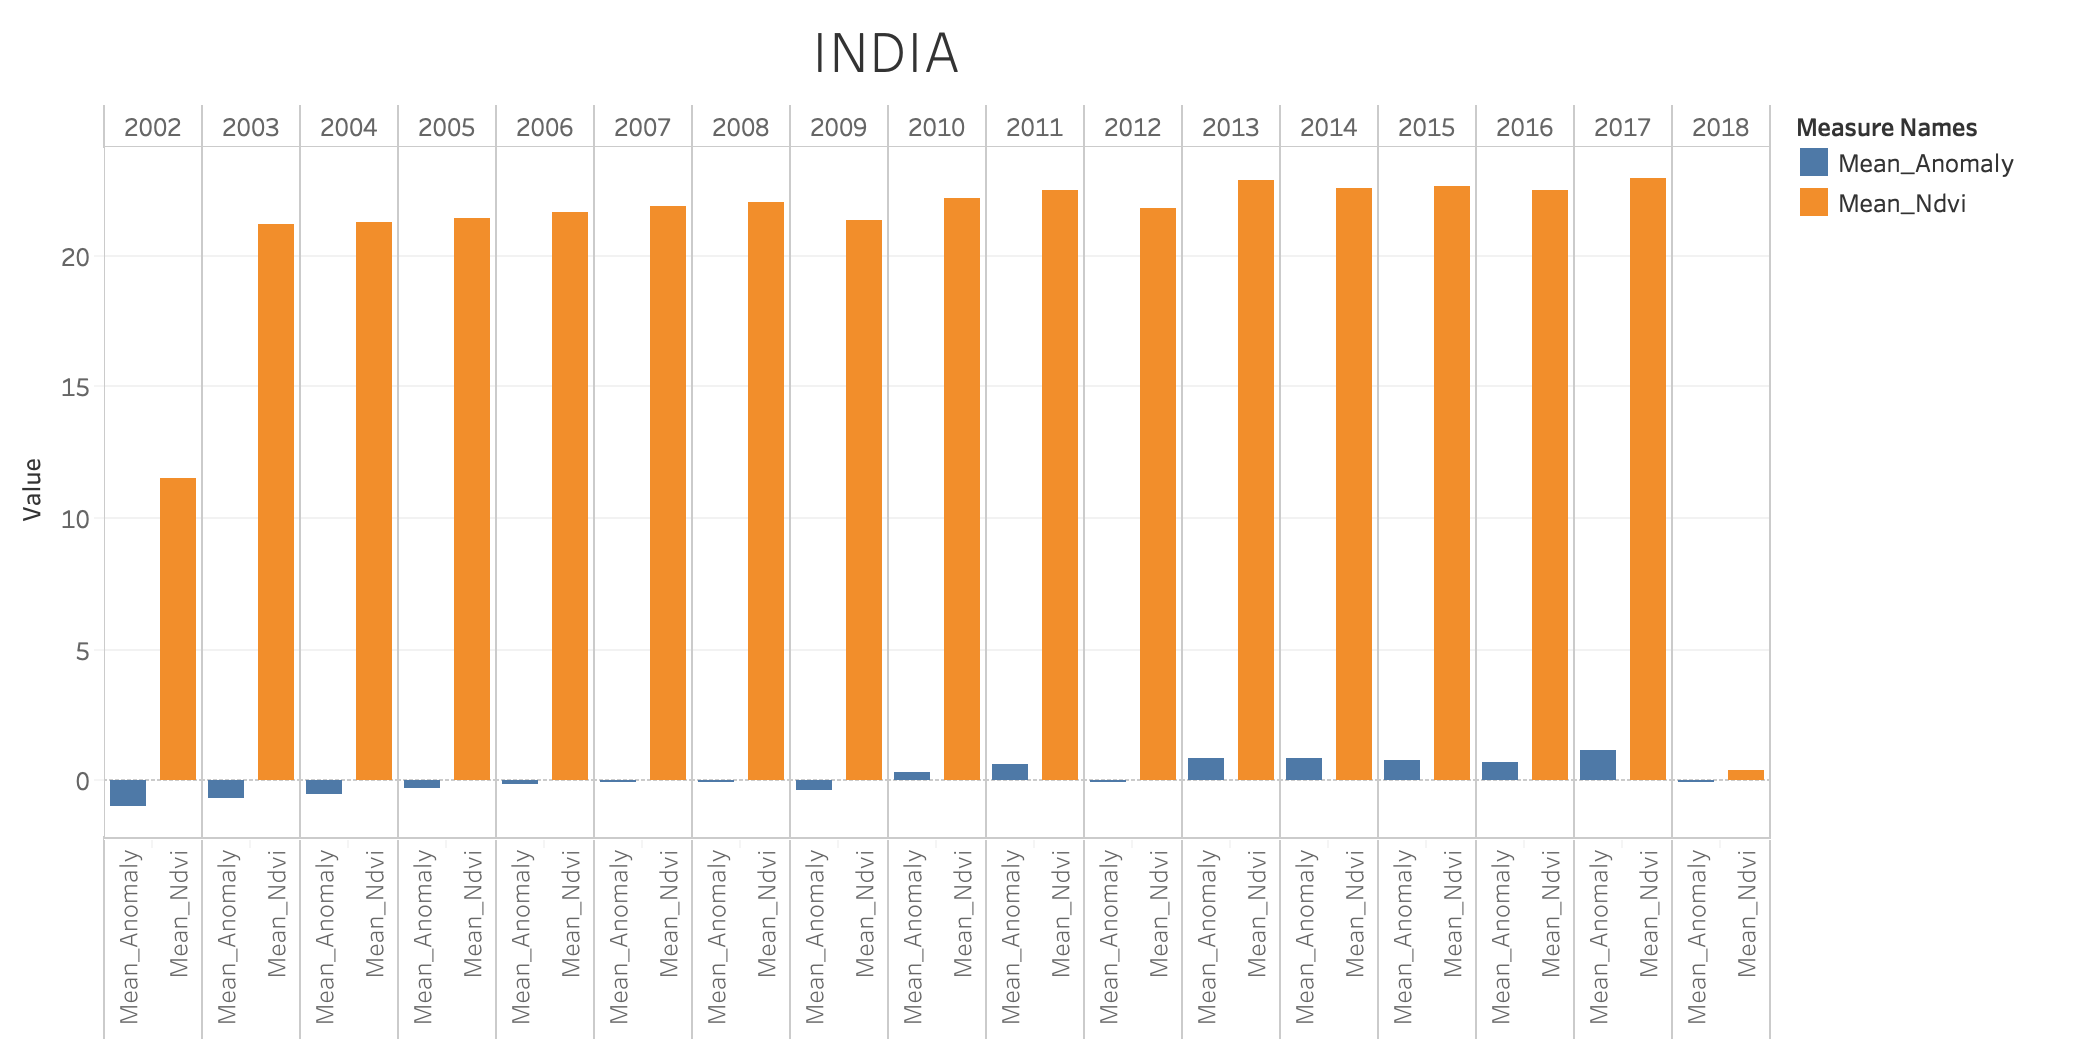
\includegraphics[width=1.0\linewidth]{figures/ch5/Histograms/INDIA_histogram.png}
            \caption{Histogram graph - India}\label{Fig:INDIA_histogram}
    \end{figure}
    
   
     \begin{figure}[H]
            \centering
            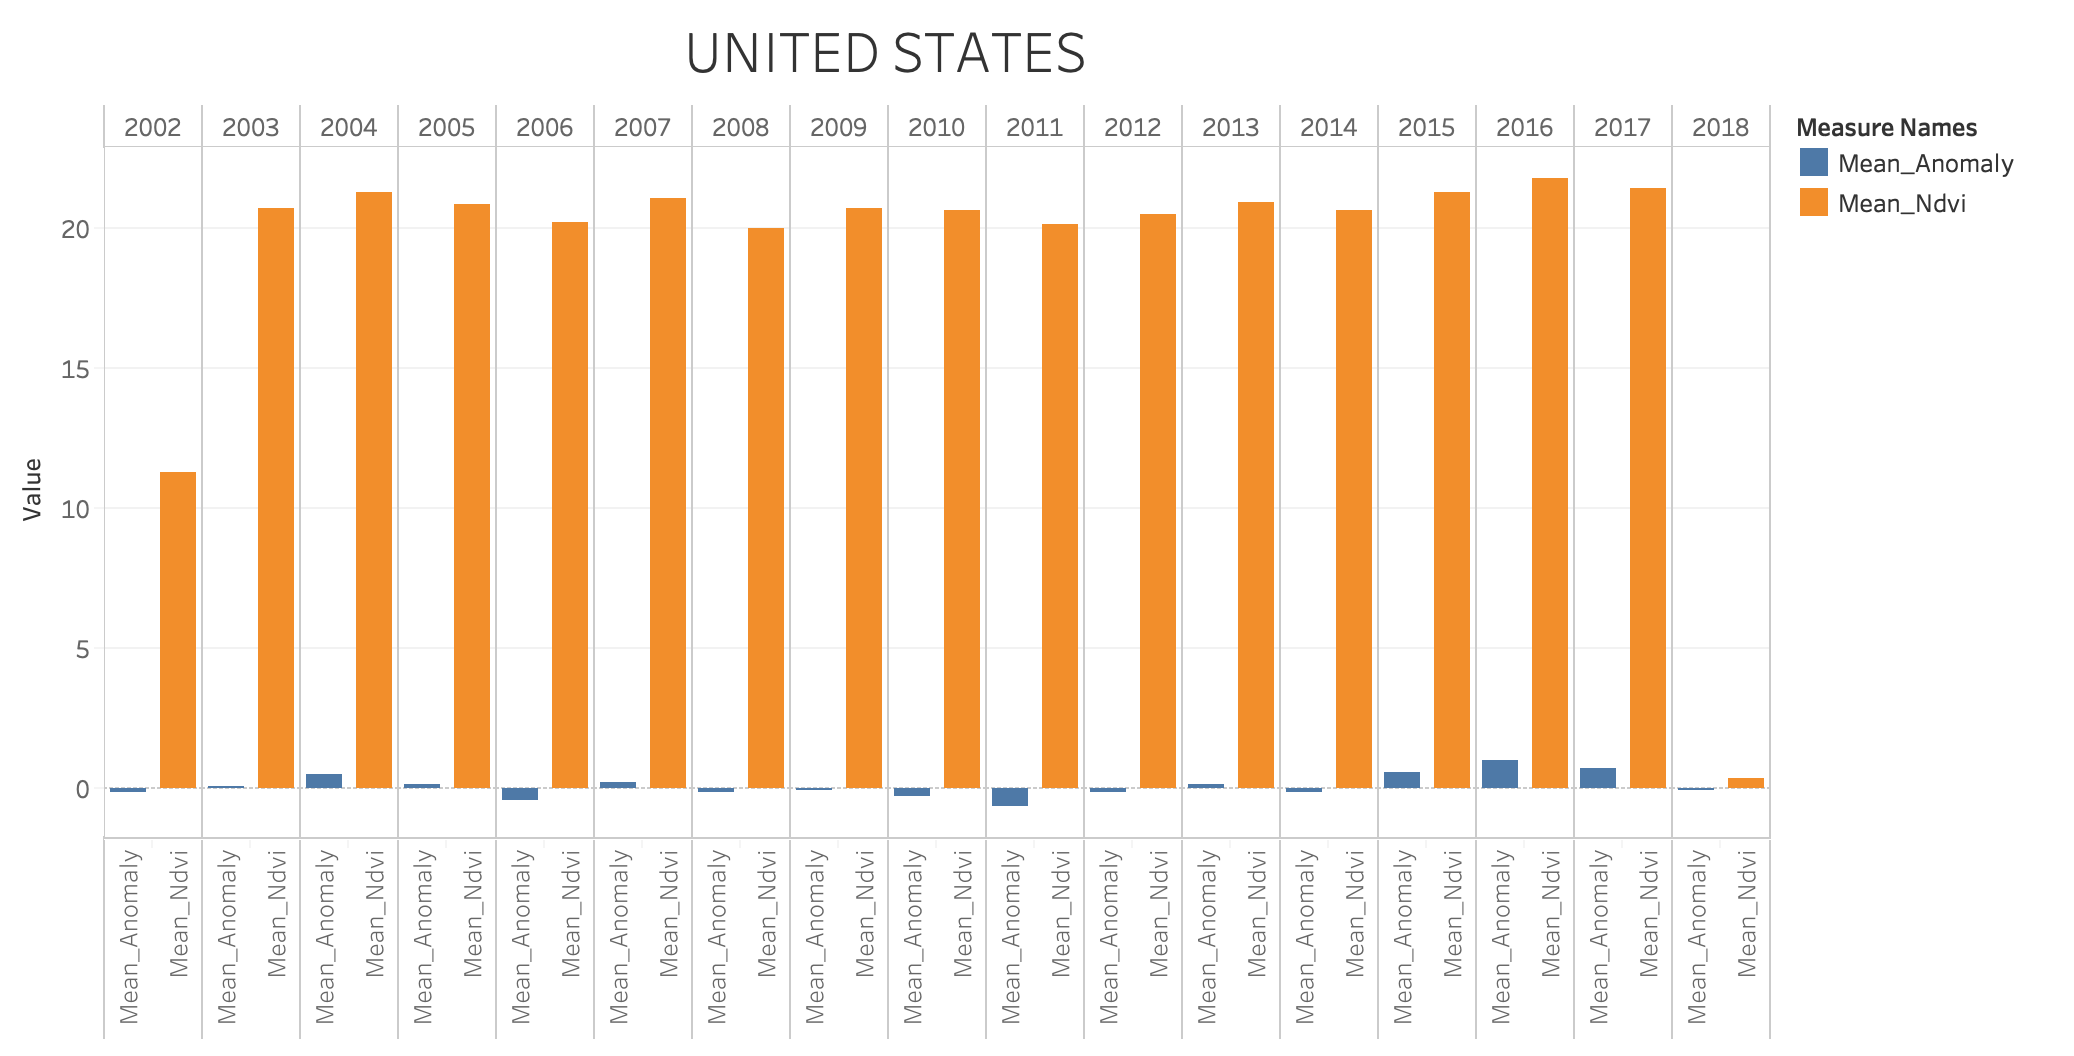
\includegraphics[width=1.0\linewidth]{figures/ch5/Histograms/US_histogram.png}
            \caption{\label{fig:US_histogram} Histogram graph - United States}
    \end{figure}
\newpage

\end{itemize}

\section{SVD Analysis}

\gls{svd} is a factorization of a real or complex matrix.  It is the generalization of the eigendecomposition of a positive semidefinite normal matrix (for example, a symmetric matrix with positive eigenvalues) to any $m$ x $n$ matrix via an extension of the polar decomposition. It has many useful applications in signal processing and statistics. \cite{SVD}

\begin{equation} \label{eq:svd_formula}
 A = UDV^{T}
\end{equation}

where $A$ is $m$ x $voin$ real matrix with $m>n$, $U$ as $m$ x $m$ and $V$ as an $n$ x $n$. Figure 5.20 shows visualisation of the matrix multiplications in \gls{svd}.

    \begin{figure}[H]
            \centering
            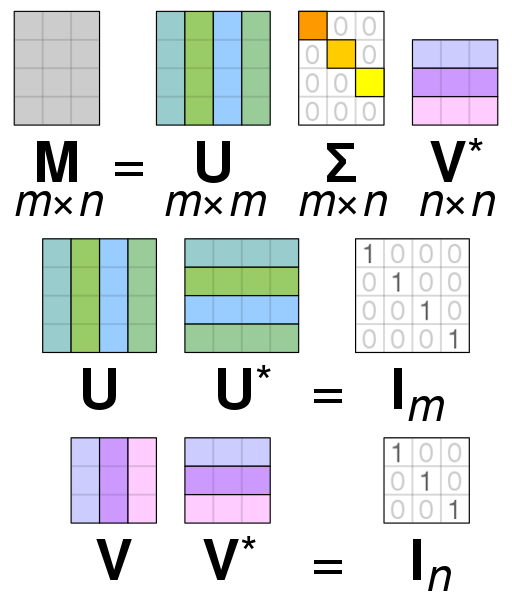
\includegraphics[width=0.5\linewidth]{figures/ch5/svd_matrix.png}
            \caption{\label{fig:svd_matrix} Matrix multiplications in SVD shown visually \cite{SVD}}
    \end{figure}

As an application, SVD is utilized to perform principle component analysis (PCA) that intends to decompose a matrix with the end goal to discover the directions (called principal axes). It also tells about the directions in which the data is distributed and is useful for dimensionality reduction. 

Steps involved in the process of implementing \gls{svd} are as follows.

\begin{itemize}
    \item Conversion of \gls{json} data into a formatted \gls{csv} file.
    \item Load the csv file in R code and remove invalid or null entries with 0.
    \item Remove the states which we don't have the data for.
    \item Plot the eigen values of \gls{ndvi} covariance matrix.
    \item Implement SVD on the matrix.
    \item Plot first five \gls{eof}'s and \gls{pca}'s.
\end{itemize}

Figure 5.21 shows the portion of snapshot of the mean \gls{ndvi} data that has been used for the analysis.

  \begin{figure}[H]
            \centering
            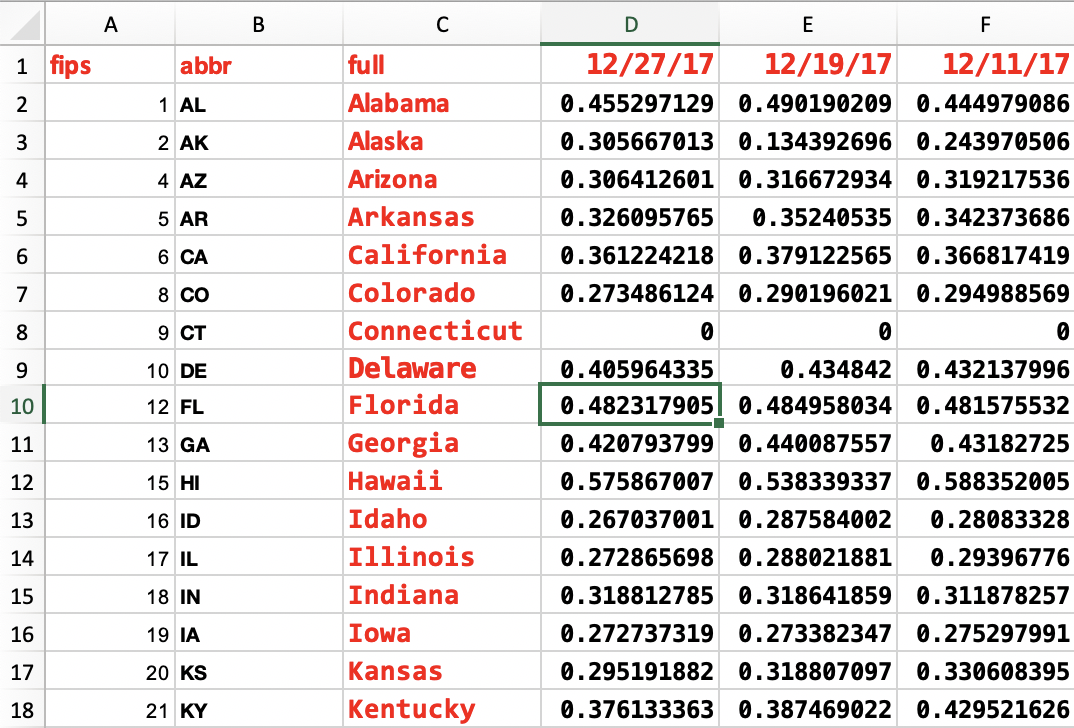
\includegraphics[width=1.0\linewidth]{figures/ch5/svd_data_snapshot.png}
            \caption{\label{fig:svd_data_snapshot} Snapshot of United States mean NDVI data of all years represented state wise}
    \end{figure}
    
\newpage    
Eigen values of \gls{ndvi} covariance matrix plot has been shown in the figure 5.22.

\begin{figure}[H]
            \centering
            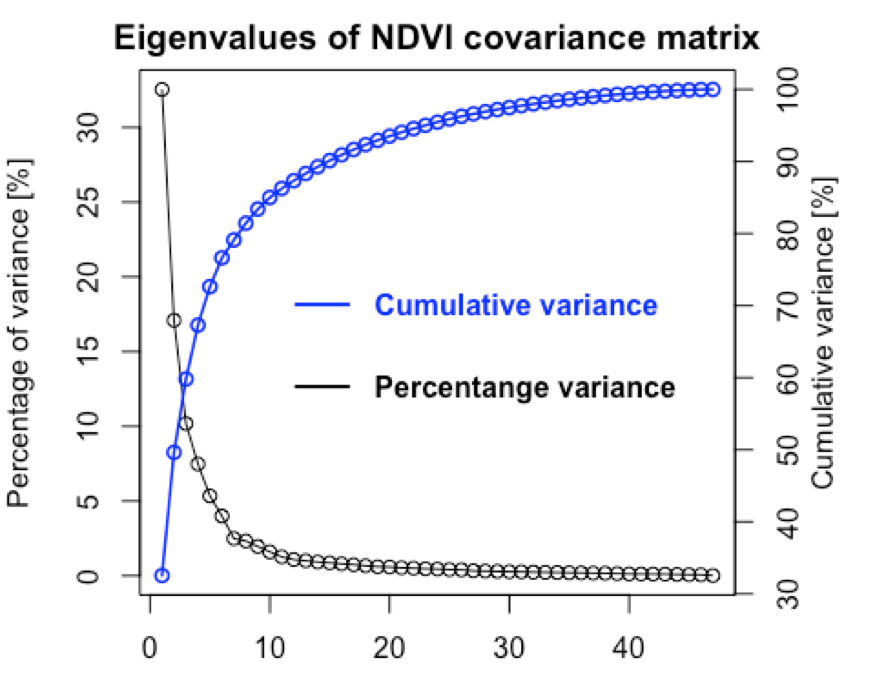
\includegraphics[width=0.70\linewidth]{figures/ch5/SVD/covarianceeigen.png}
            \caption{\label{fig:covriance} Eigen values of NDVI covariance matrix.}
    \end{figure}


The size of $A$ matrix is $47$ x $714$, column belongs to dates and row for states. After applying \gls{svd} to matrix $A$, the matrices, $U$, $D$ and $VT$ are shown below in figure 5.23.

    \begin{figure}[H]
            \centering
            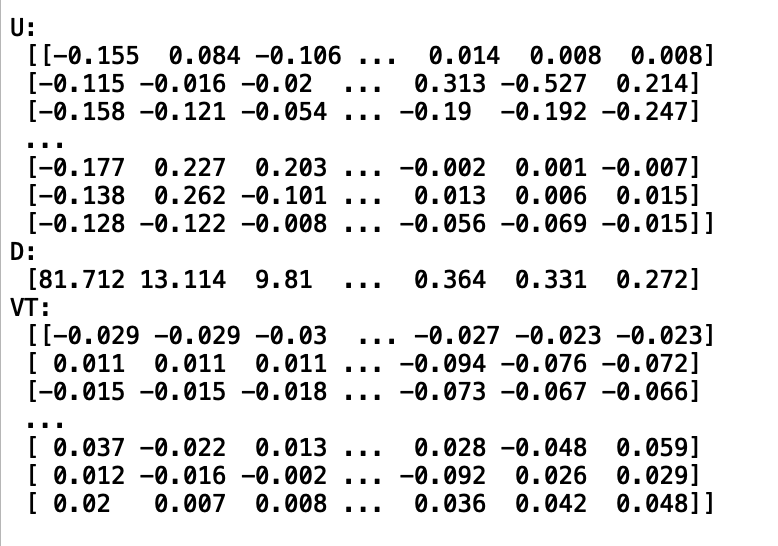
\includegraphics[width=0.70\linewidth]{figures/ch5/svd_result_matrix.png}
            \caption{\label{fig:svd_result_matrices} Result of SVD on matrix A - U, D \& VT}
    \end{figure}
    
    \gls{eof}s and \gls{pca}s plots of first five vectors has been shown in below figures.
    
     \begin{figure}[H]
            \centering
            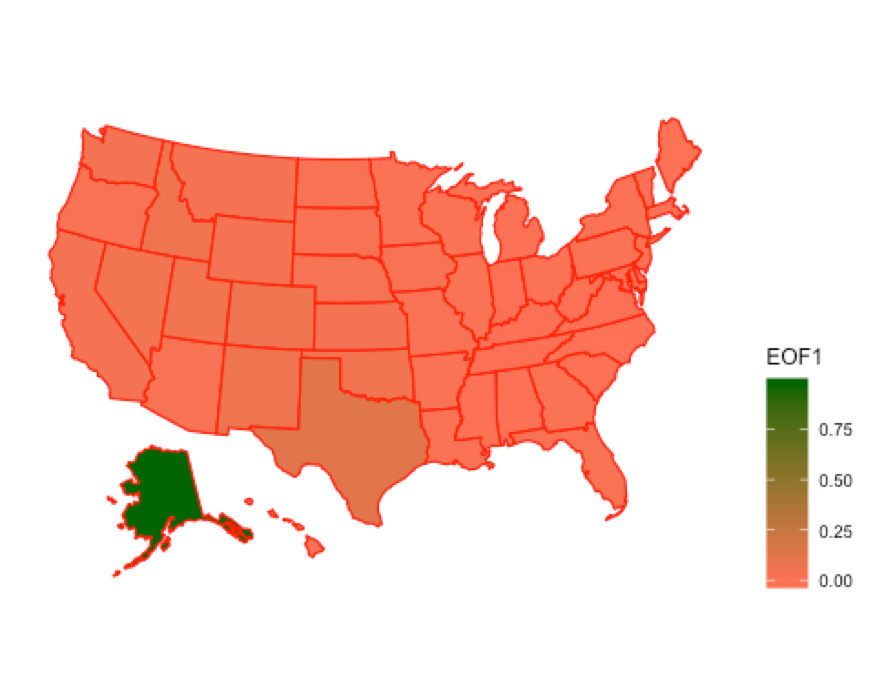
\includegraphics[width=0.70\linewidth]{figures/ch5/SVD/eof1.png}
            \caption{\label{fig:EOF_1} Mask mapping state wise of U1 vector of matrix U}
    \end{figure}
    
     \begin{figure}[H]
            \centering
            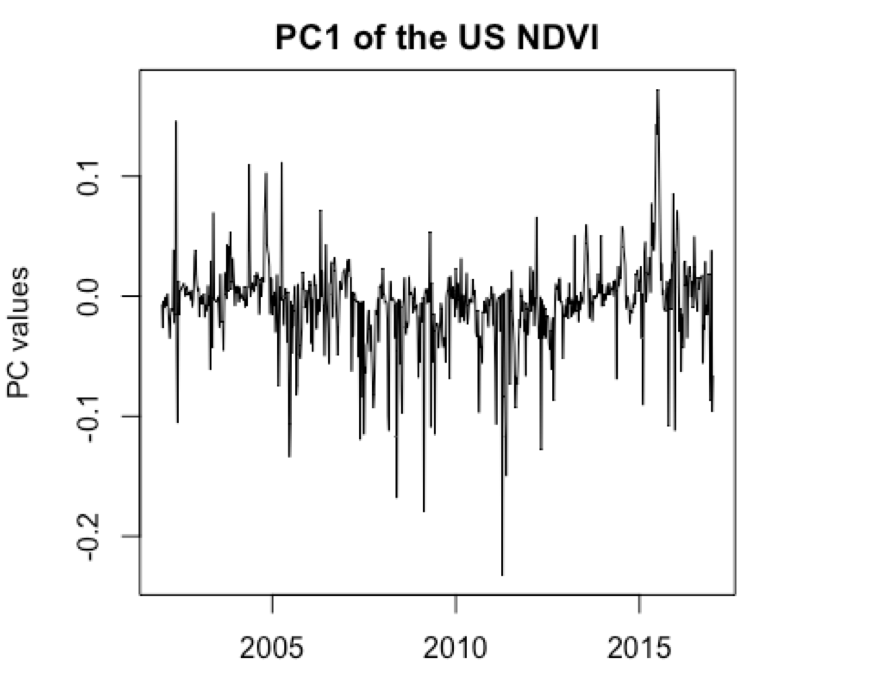
\includegraphics[width=0.70\linewidth]{figures/ch5/SVD/pc1.png}
            \caption{\label{fig:V_1} Time series analysis of V1 vector of matrix V}
    \end{figure}
    
    \begin{figure}[H]
            \centering
            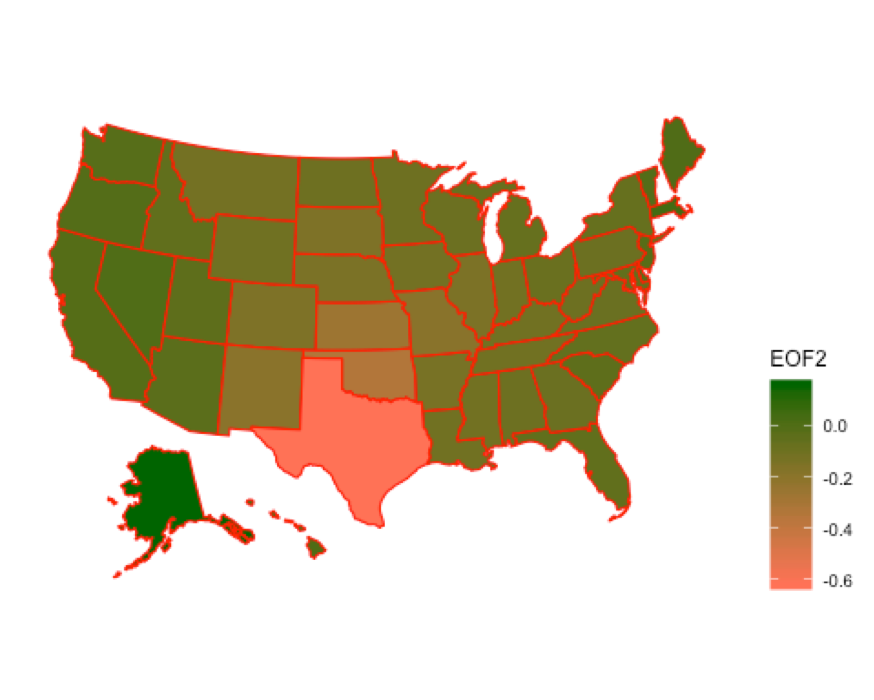
\includegraphics[width=0.70\linewidth]{figures/ch5/SVD/eof2.png}
            \caption{\label{fig:EOF_2} Mask mapping state wise of U2 vector of matrix U}
    \end{figure}
    
    \begin{figure}[H]
            \centering
            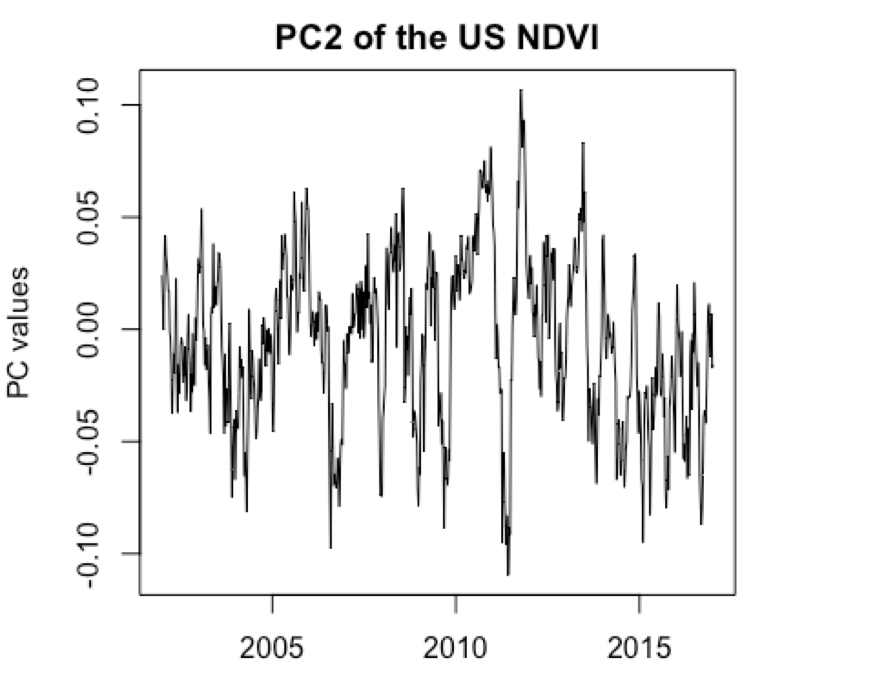
\includegraphics[width=0.70\linewidth]{figures/ch5/SVD/pc2.png}
            \caption{\label{fig:V_2} Time series analysis of V2 vector of matrix V}
    \end{figure}
    
     \begin{figure}[H]
            \centering
            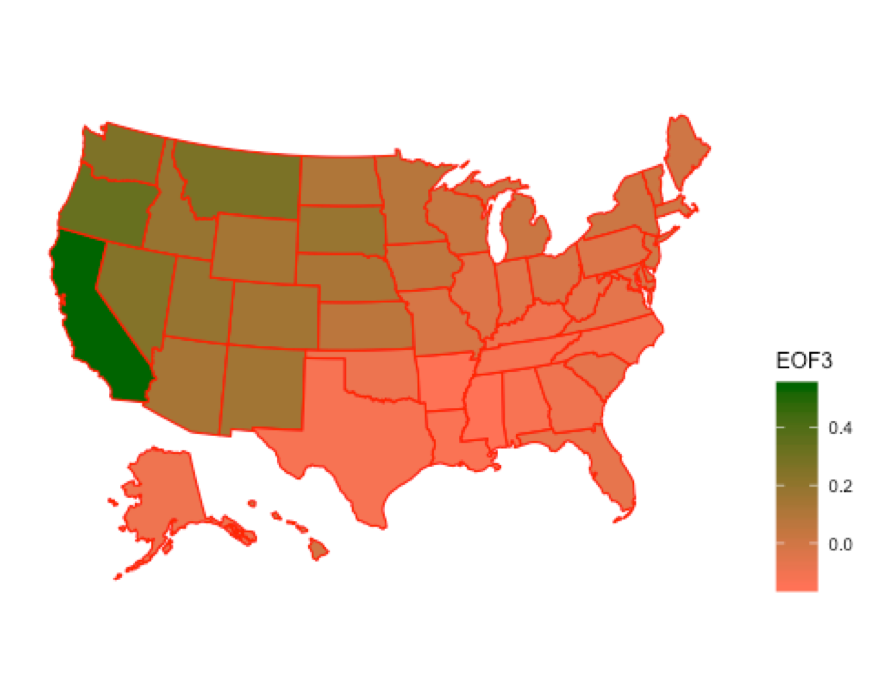
\includegraphics[width=0.70\linewidth]{figures/ch5/SVD/eof3.png}
            \caption{\label{fig:EOF_3} Mask mapping state wise of U3 vector of matrix U}
    \end{figure}
    
     \begin{figure}[H]
            \centering
            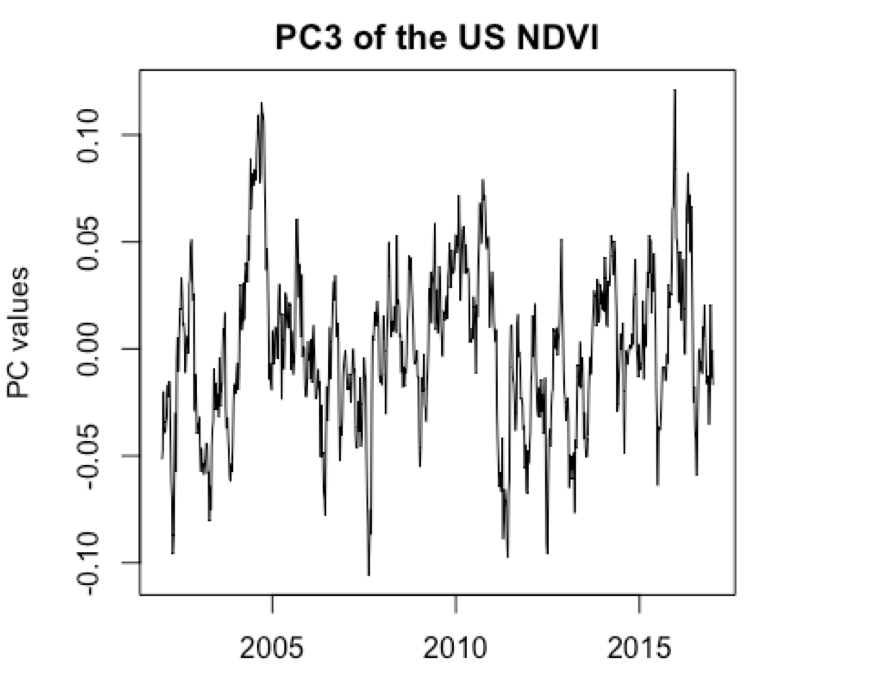
\includegraphics[width=0.70\linewidth]{figures/ch5/SVD/pc3.png}
            \caption{\label{fig:V_3} Time series analysis of V3 vector of matrix V}
    \end{figure}
    
    
     \begin{figure}[H]
            \centering
            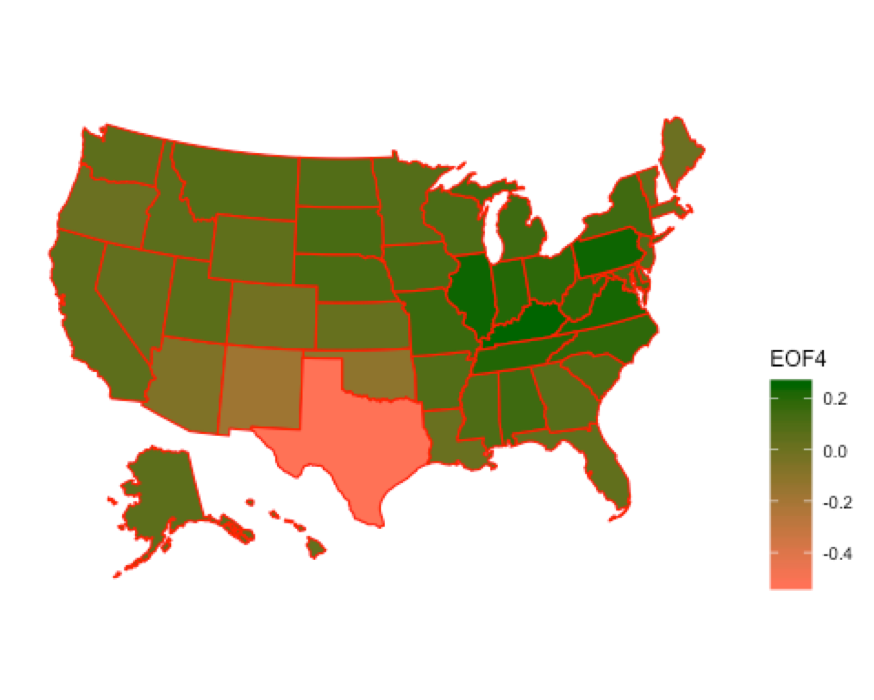
\includegraphics[width=0.70\linewidth]{figures/ch5/SVD/eof4.png}
            \caption{\label{fig:EOF_4} Mask mapping state wise of U4 vector of matrix U}
    \end{figure}
    
     \begin{figure}[H]
            \centering
            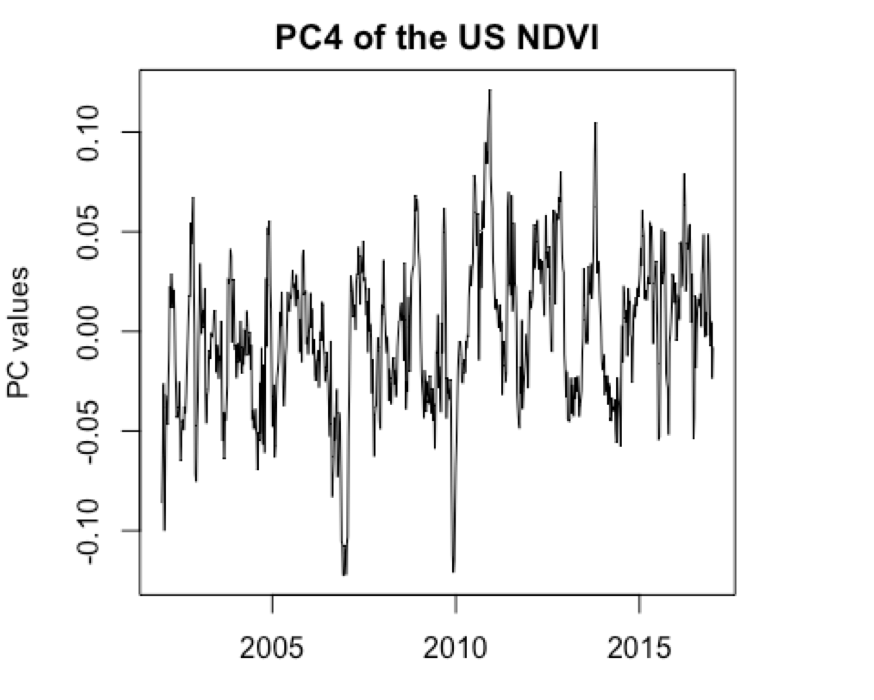
\includegraphics[width=0.70\linewidth]{figures/ch5/SVD/pc4.png}
            \caption{\label{fig:V_4} Time series analysis of V4 vector of matrix V}
    \end{figure}
    
    
     \begin{figure}[H]
            \centering
            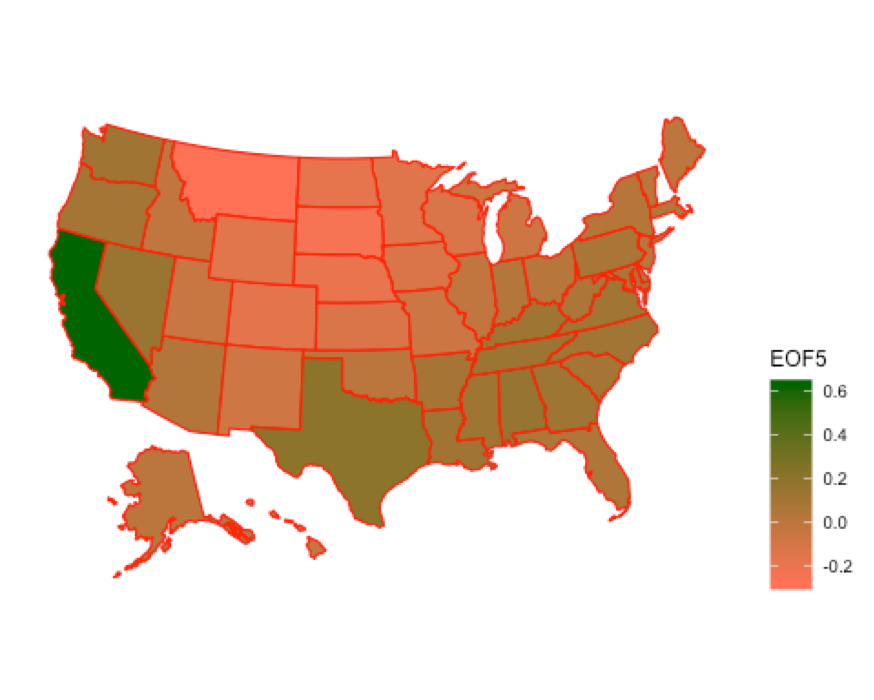
\includegraphics[width=0.70\linewidth]{figures/ch5/SVD/eof5.png}
            \caption{\label{fig:EOF_5} Mask mapping state wise of U5 vector of matrix U}
    \end{figure}
    
     \begin{figure}[H]
            \centering
            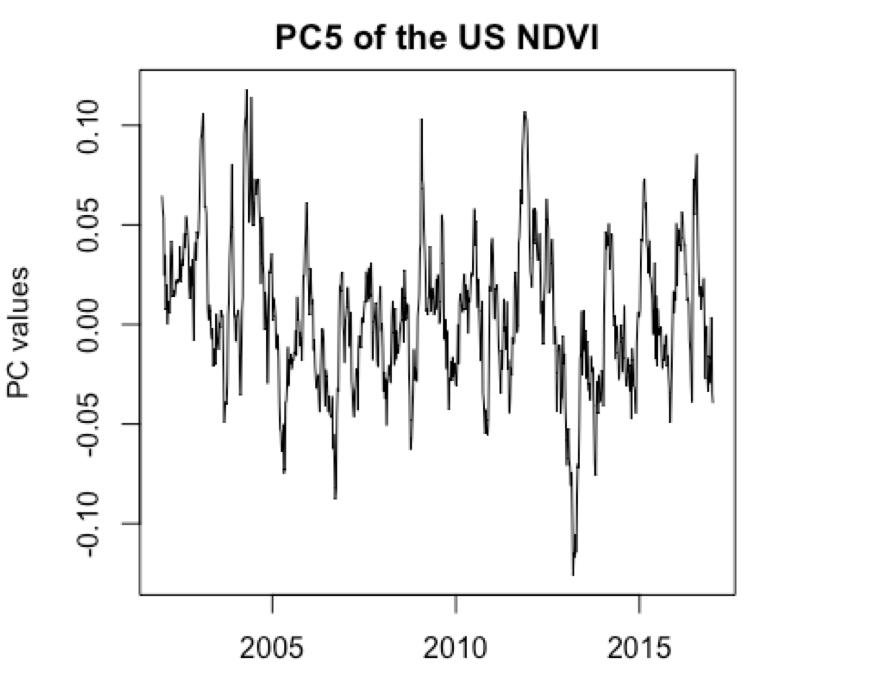
\includegraphics[width=0.70\linewidth]{figures/ch5/SVD/pc5.png}
            \caption{\label{fig:V_5} Time series analysis of V5 vector of matrix V}
    \end{figure}